%%%%%%%%%%%%%%%%%%%%%%%%%%%%%%%%%%%%%%%%%
% Beamer Presentation
%%%%%%%%%%%%%%%%%%%%%%%%%%%%%%%%%%%%%%%%%

%----------------------------------------------------------------------------------------
% CLASSE DO DOCUMENTO
%----------------------------------------------------------------------------------------

\documentclass[
    11pt,
    %aspectratio=169
]{beamer}

%----------------------------------------------------------------------------------------
% CAMINHO DAS IMAGENS
%----------------------------------------------------------------------------------------

\graphicspath{{img/}}

%----------------------------------------------------------------------------------------
% PACOTES
%----------------------------------------------------------------------------------------

\usepackage{
    booktabs,
    multirow,
    palatino,
    subcaption
}

\usepackage[default]{opensans}

\usepackage{tikz}
\usepackage{xcolor}
\usepackage{pifont}
\usepackage{hyperref}

\hypersetup{
    hidelinks,
    urlcolor=blue
}

\input{config/code_langs}

%----------------------------------------------------------------------------------------
% BIBLIOGRAFIA
%----------------------------------------------------------------------------------------

\usepackage[backend=biber,style=numeric]{biblatex}
\addbibresource{bibliografia.bib}

%----------------------------------------------------------------------------------------
% TEMA
%----------------------------------------------------------------------------------------

\usetheme{Boadilla}
\useinnertheme{circles}
\useoutertheme{smoothbars}
\usecolortheme{dove}
\usefonttheme{professionalfonts}

\setbeamertemplate{navigation symbols}{}
\setbeamertemplate{sections/subsections in toc}[sections numbered]

%----------------------------------------------------------------------------------------
% CORES
%----------------------------------------------------------------------------------------

\definecolor{primaryColor}{RGB}{46,78,102}
\definecolor{secondaryColor}{RGB}{224,231,236}
\definecolor{thirdColor}{RGB}{92,118,138}
\definecolor{accentColor}{RGB}{122,146,164}
\definecolor{textColor}{RGB}{35,44,52}
\definecolor{titleRed}{RGB}{132,42,42}

%----------------------------------------------------------------------------------------
% CONFIGURAÇÃO DAS CORES DO BEAMER
%----------------------------------------------------------------------------------------

\setbeamercolor{structure}{fg=primaryColor}
\setbeamercolor{normal text}{fg=textColor,bg=white}
\setbeamercolor{background canvas}{bg=white}

\setbeamercolor{palette primary}{
    bg=primaryColor,
    fg=white
}

\setbeamercolor{palette secondary}{
    bg=secondaryColor,
    fg=textColor
}

\setbeamercolor{palette tertiary}{
    bg=thirdColor,
    fg=white
}

\setbeamercolor{palette quaternary}{
    bg=secondaryColor,
    fg=textColor
}

\setbeamercolor{title}{
    fg=white,
    bg=primaryColor
}

\setbeamercolor{frametitle}{
    fg=primaryColor,
    bg=secondaryColor
}

\setbeamercolor{block title}{
    fg=white,
    bg=thirdColor
}

\setbeamercolor{block body}{
    fg=textColor,
    bg=secondaryColor!45!white
}

%----------------------------------------------------------------------------------------
% CABEÇALHO E RODAPÉ
%----------------------------------------------------------------------------------------

\setbeamercolor{headline}{
    bg=secondaryColor,
    fg=textColor
}

\setbeamercolor{author in head/foot}{
    bg=primaryColor,
    fg=white
}

\setbeamercolor{title in head/foot}{
    bg=thirdColor,
    fg=white
}

\setbeamercolor{date in head/foot}{
    bg=primaryColor,
    fg=white
}

\setbeamercolor{section in head/foot}{
        bg=secondaryColor,
        fg=textColor
}

\setbeamercolor{section in head/foot shaded}{
        bg=secondaryColor,
        fg=accentColor
}

\setbeamerfont{title}{series=\bfseries}
\setbeamerfont{frametitle}{series=\bfseries,size=\large}

\setbeamertemplate{headline}{%
    \begin{beamercolorbox}[wd=\paperwidth,ht=3.1ex,dp=1.4ex,leftskip=0.8cm,rightskip=0.3cm]{section in head/foot}
        \insertsectionnavigationhorizontal{\dimexpr\paperwidth-1.1cm\relax}{}{}
    \end{beamercolorbox}%
}

\setbeamertemplate{footline}{%
    \leavevmode%
    \hbox{%
        \begin{beamercolorbox}[wd=.72\paperwidth,ht=2.8ex,dp=1.2ex,leftskip=0.8cm]{author in head/foot}%
            \usebeamerfont{author in head/foot}\insertshortauthor\hfill\insertshorttitle
        \end{beamercolorbox}%
        \begin{beamercolorbox}[wd=.28\paperwidth,ht=2.8ex,dp=1.2ex,rightskip=0.8cm plus1fil]{date in head/foot}%
            \usebeamerfont{date in head/foot}\hfill\insertframenumber\,/\,\inserttotalframenumber
        \end{beamercolorbox}%
    }%
}

%----------------------------------------------------------------------------------------
% COMANDOS PERSONALIZADOS
%----------------------------------------------------------------------------------------

\newcommand{\done}{
    \textcolor{green}{\ding{51}}
}

\newcommand{\blocked}{
    \textcolor{red}{\ding{55}}
}

\newcommand{\pending}{%
  \tikz[baseline=-0.6ex]
  \draw[gray!70, line width=0.5pt]
  (0,0) circle (0.7ex);
}

\newcommand{\inprogress}{%
  \tikz[baseline=-0.6ex]{
    \draw[blue!70!black, line width=0.5pt]
    (0,0) circle (0.7ex);

    \fill[blue!70!black]
      (0,0) --
      (0,0.7ex)
      arc (90:-70:0.7ex)
      -- cycle;
  }
}

%----------------------------------------------------------------------------------------
% INFORMAÇÕES DA APRESENTAÇÃO
%----------------------------------------------------------------------------------------

\title[Experimental Correlated Uncertainty]
{
Exploring the universality of scaled particle spectra\\
with Bayesian inference in heavy-ion collisions
}

\author[Nara Moraes]
{
\textbf{Nara Avila Moraes}
}

\institute[IFUSP]
{
Advisor: \textbf{Prof. Dr. Matthew William Luzum}\\[0.2cm]
Instituto de Física da Universidade de São Paulo (IFUSP)\\[0.2cm]
Supported by CNPq
}

\date[2026]
{
XXXIII Reunião de Trabalho sobre Interações Hadrônicas\\
June 24, 2026
}

%----------------------------------------------------------------------------------------
% INÍCIO DO DOCUMENTO
%----------------------------------------------------------------------------------------

\begin{document}

%----------------------------------------------------------------------------------------
% CAPA
%----------------------------------------------------------------------------------------

\begin{frame}[plain]

\begin{center}

\vspace{0.3cm}

%-----------------------------------
% TÍTULO
%-----------------------------------

{\LARGE
\textcolor{titleRed}{
\textbf{
Study of the effect of correlated experimental uncertainty on Bayesian
Inference of quark–gluon plasma properties
}
}
}

\vspace{0.5cm}

%-----------------------------------
% REFERÊNCIA
%-----------------------------------
\vspace{0.5cm}

%-----------------------------------
% AUTOR
%-----------------------------------

{\Large
\textbf{M.Sc. student: Nara Moraes}
}

\vspace{0.3cm}

%-----------------------------------
% ORIENTADOR
%-----------------------------------

{\large
Advisor: \textbf{Prof. Dr. Matthew William Luzum}
}

\vspace{0.3cm}

%-----------------------------------
% AFILIAÇÃO
%-----------------------------------



\vspace{0.5cm}

%-----------------------------------
% EVENTO
%-----------------------------------

{\large
XXXIII Reunião de Trabalho sobre Interações Hadrônicas\\
}

\vspace{0.15cm}

{\large
June 26, 2026
}

\vfill

%-----------------------------------
% LOGOS
%-----------------------------------

\begin{figure}
\centering

\includegraphics[height=1cm]{logo_ifusp.png}
\hspace{0.5cm}

\includegraphics[height=1.2cm]{logo_ifna.png}
\hspace{0.5cm}

\includegraphics[height=1.1cm]{logo_cbpf.jpg}
\hspace{0.5cm}
\raisebox{1mm}{
\includegraphics[height=0.9cm]{logo_cnpq.jpg}}

\end{figure}

\end{center}

\end{frame}

%----------------------------------------------------------------------------------------
% SUMÁRIO
%----------------------------------------------------------------------------------------

\begin{frame}
    \frametitle{Outline}
    \tableofcontents
\end{frame}

%----------------------------------------------------------------------------------------
% SEÇÕES
%----------------------------------------------------------------------------------------


\section{Motivation: Quark--Gluon Plasma}
\begin{frame}
\frametitle{Motivation: Probing the Quark--Gluon Plasma}

\begin{columns}[T]

\column{0.52\textwidth}

\small
Relativistic heavy-ion collisions create extreme conditions of temperature and energy density, where nuclear matter undergoes a transition to a deconfined state of quarks and gluons: the Quark--Gluon Plasma (QGP).

\vspace{0.25cm}

Our goal is to constrain the properties of this medium from experimental data, especially:

\begin{itemize}
    \item the initial energy density and geometry;
    \item the QGP transport properties, such as shear and bulk viscosity;
    \item the hydrodynamic evolution and freeze-out conditions;
    \item the connection between model parameters and final hadron spectra.
\end{itemize}

\vspace{0.15cm}

Bayesian calibration allows us to compare full collision simulations with measured observables and infer the most probable QGP parameters.

\column{0.48\textwidth}

\centering
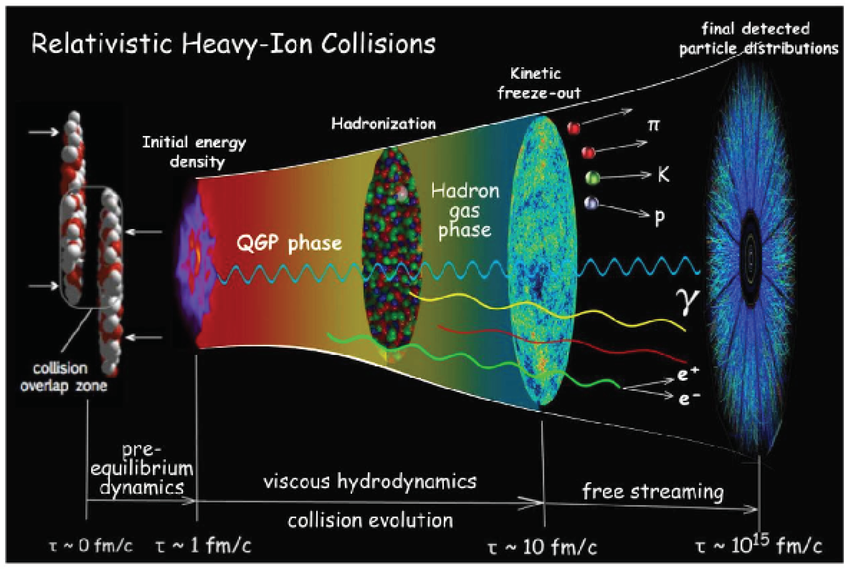
\includegraphics[width=\linewidth]{img/qgp.png}

\vspace{0.1cm}
{\tiny Schematic evolution of a relativistic heavy-ion collision.}

\end{columns}
\end{frame}


%--------------------------------------------------------
\begin{frame}
\frametitle{Baryon Enhancement}

\begin{columns}[T,onlytextwidth]

%--------------------------------------------------------
\column{0.38\textwidth}

\small

\textbf{Observable}

\[
\frac{p}{\pi}(p_T)
=
\frac{dN_p/dp_T}{dN_\pi/dp_T}
\]

\vspace{0.25cm}

\textbf{Enhancement region}

\[
2 \lesssim p_T \lesssim 5~{\rm GeV}/c
\]

\vspace{0.4cm}

\begin{itemize}
    \item Larger in central Pb--Pb.
    \item Driven by collective radial flow.
    \item Sensitive to QGP hadronization.
\end{itemize}

{\tiny
Data source: HEPData\\
10.17182/HEPData-ins1759506-v1.
}
%--------------------------------------------------------
\column{0.60\textwidth}

\centering

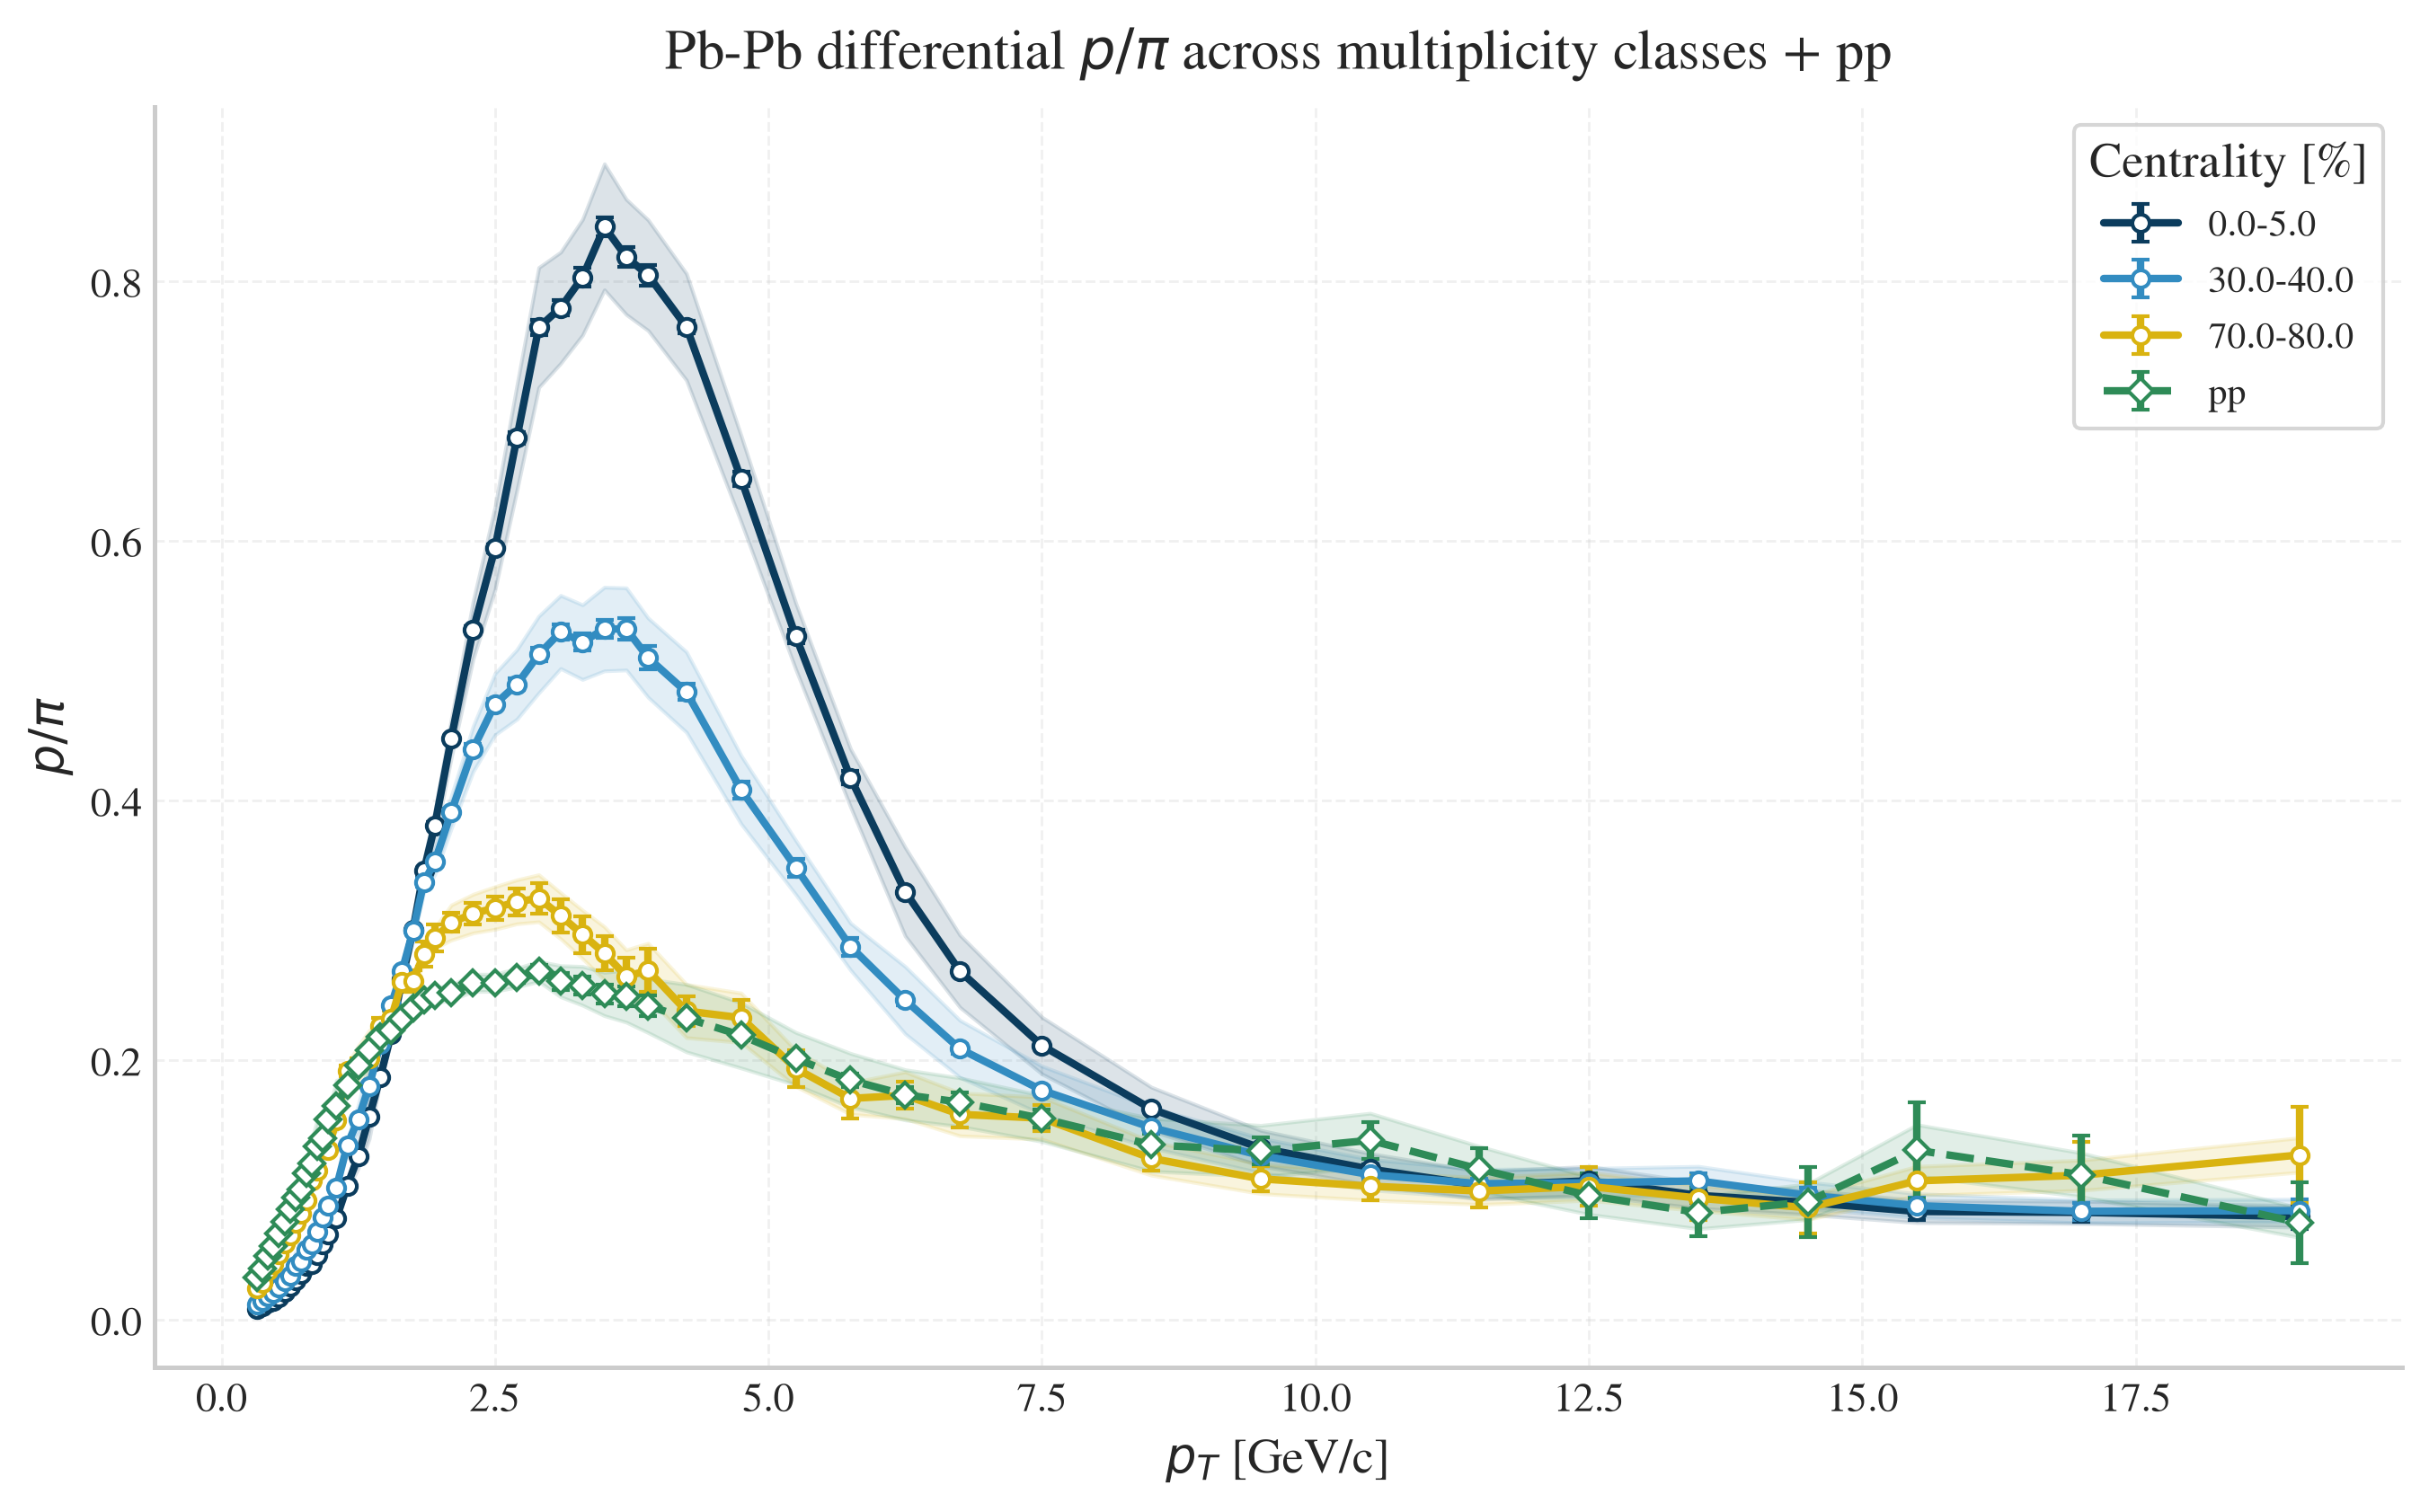
\includegraphics[
    width=\linewidth,
    height=0.45\textheight,
    keepaspectratio
]{img/qgp-enhancement.png}

\vspace{-0.3cm}
\begin{block}{Quark coalescence}
\small
The high quark density in the QGP favors hadronization by quark
recombination,
\[
qqq \rightarrow p,
\quad
q\bar q \rightarrow \pi ,
\]

enhancing baryon production relative to mesons at intermediate $p_T$.
\end{block}

\vspace{0.05cm}

{\tiny Differential $p/\pi$ ratio for different Pb--Pb centralities.}

\end{columns}

\vfill

\end{frame}
%--------------------------------------------------------
\begin{frame}
\frametitle{Nuclear Suppression}

\begin{columns}[T,onlytextwidth]

%--------------------------------------------------------
% Left
%--------------------------------------------------------

\column{0.52\textwidth}

\centering
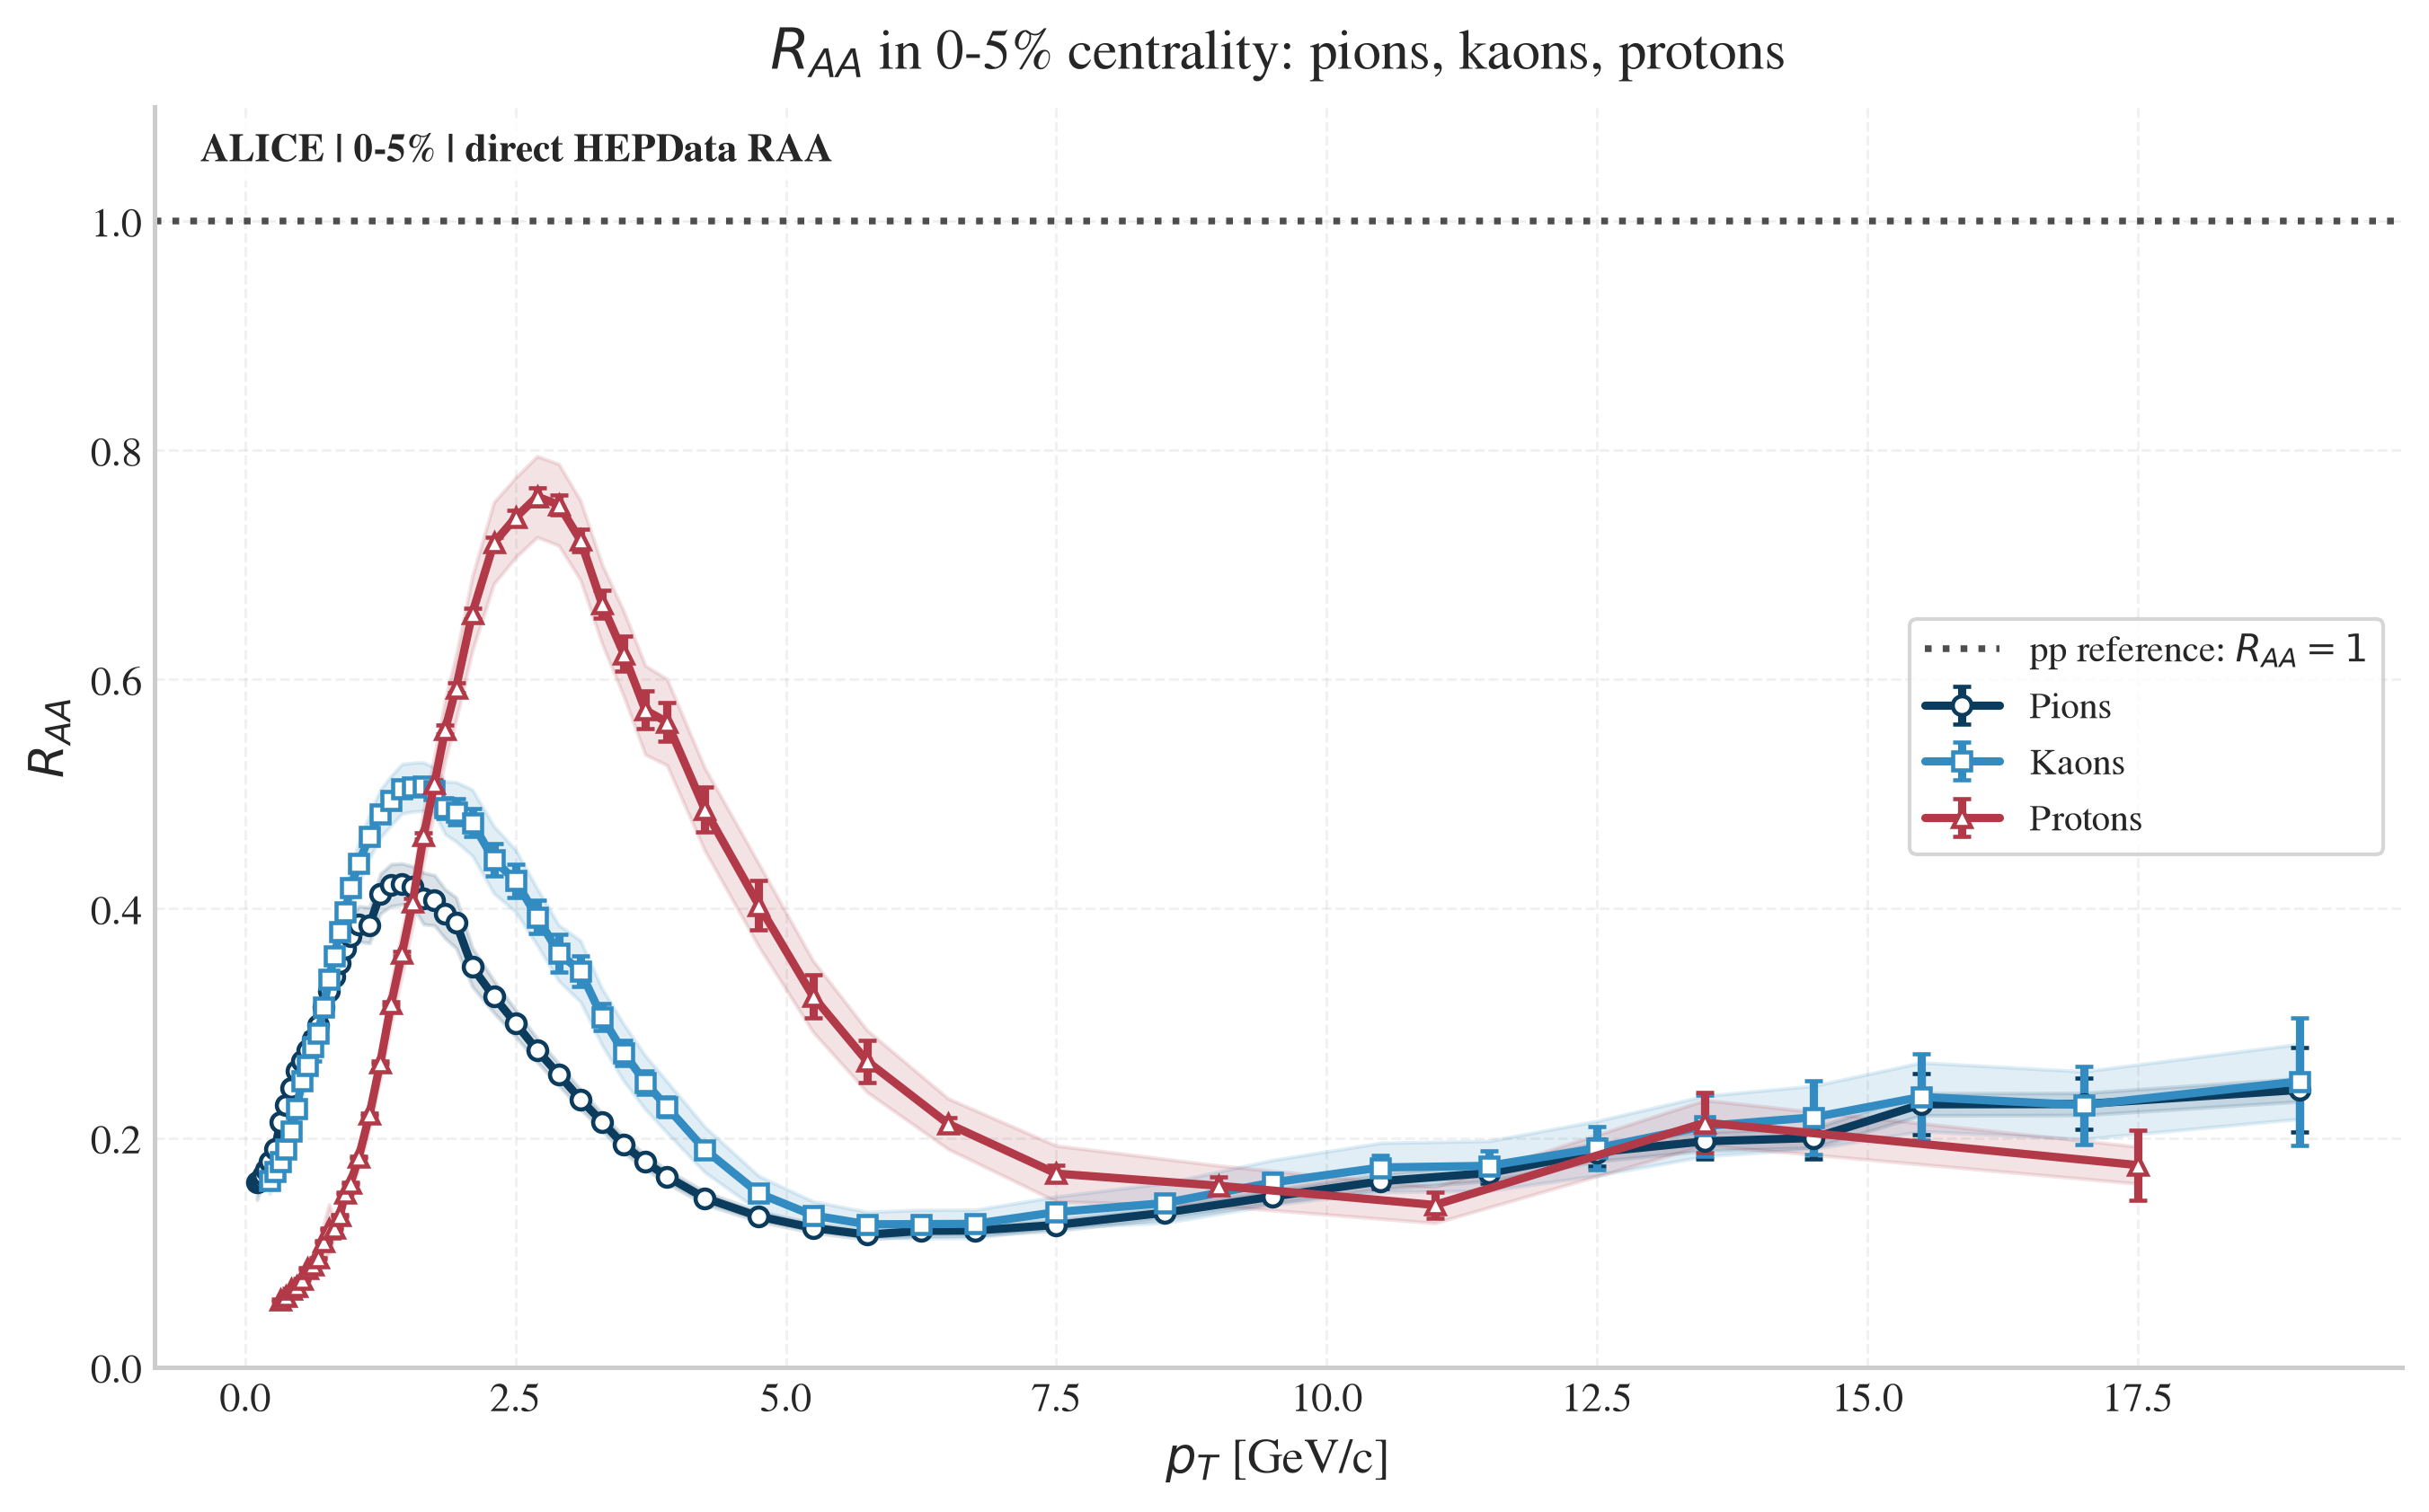
\includegraphics[width=\linewidth]{img/qgp-nuclear-supression.png}

\begin{block}{Jet quenching}
\small
Hard-scattered partons lose energy while traversing the QGP through
multiple interactions with the medium. As a consequence, fewer
high-$p_T$ hadrons are reconstructed, leading to
$R_{AA}<1$.
\end{block}

{\tiny Data source: HEPData 10.17182/HEPData-ins1759506-v1.}

%--------------------------------------------------------
% Right
%--------------------------------------------------------

\column{0.44\textwidth}

\small

\textbf{Nuclear modification factor}

\vspace{-0.15cm}

\[
R_{AA}(p_T)=
\frac{1}{\langle N_{\rm coll}\rangle}
\frac{dN_{AA}/dp_T}
{dN_{pp}/dp_T}
\]

\vspace{0.6cm}


\begin{itemize}
\item $R_{AA}=1$: binary collision scaling.

\item $R_{AA}<1$: suppression due to medium-induced energy loss.

\item Intermediate $p_T$: protons are less suppressed than mesons.

\item High $p_T$: all hadron species exhibit a similar suppression.
\end{itemize}

\end{columns}

\end{frame}
\section{Bayesian Analysis}

%--------------------------------------------------------
\begin{frame}
\frametitle{Bayesian Parameter Estimation}

\small

The properties of the QGP are not directly observable; they are inferred by
comparing theoretical predictions with experimental measurements.

\vspace{0.15cm}

\begin{columns}[T]

%--------------------------------------------------------
\column{0.50\textwidth}

Bayes' theorem updates prior knowledge using experimental evidence:

\[
P(\boldsymbol{\theta}|D)
\propto
P(D|\boldsymbol{\theta})P(\boldsymbol{\theta})
\]

\begin{itemize}
    \item $\boldsymbol{\theta}$: model parameters
    \item $P(\boldsymbol{\theta})$: prior
    \item $P(D|\boldsymbol{\theta})$: likelihood
    \item $P(\boldsymbol{\theta}|D)$: posterior
\end{itemize}

{\tiny
J. E. Bernhard, J. S. Moreland and S. A. Bass,
\textit{Bayesian estimation of the specific shear and bulk viscosity of quark--gluon plasma},
Nature Physics \textbf{15}, 1113--1117 (2019).
}
%--------------------------------------------------------
\column{0.50\textwidth}

\centering
\footnotesize

\[
\boxed{\text{Experimental Data}}
\hspace{0.6cm}
\boxed{\text{Model Predictions}}
\]

\[
\searrow
\hspace{2.0cm}
\swarrow
\]

\[
\boxed{\text{Likelihood}}
\]

\[
\Downarrow
\]

\[
\boxed{\text{Posterior}}
\]

Sampled through MCMC.

\end{columns}

\vfill

\end{frame}
%------------------------------------------------------
--
\section{Likelihood and Uncertainty Quantification}
\begin{frame}
\frametitle{Likelihood and Uncertainty Quantification}

\small

The agreement between model predictions and experimental data is quantified
through a multivariate Gaussian likelihood:

\vspace{0.2cm}

\[
\mathcal{L}(\boldsymbol{\theta})
=
\frac{1}
{\sqrt{(2\pi)^n |\Sigma|}}
\exp\left[
-\frac12
(\mathbf y_m-\mathbf y_e)^T
\Sigma^{-1}
(\mathbf y_m-\mathbf y_e)
\right]
\]

\vspace{0.2cm}

where

\[
\Sigma=\Sigma_{\rm exp}+\Sigma_{\rm model}.
\]

\vspace{0.2cm}

\begin{columns}[T]

\column{0.48\textwidth}

\textbf{Experimental uncertainty}

\[
\Sigma_{\rm exp}
=
\Sigma_{\rm stat}^{\rm exp}
+
\Sigma_{\rm sys}^{\rm exp}
\]

\begin{itemize}
\item Statistical uncertainty
\item Correlated systematic uncertainty
\end{itemize}

\column{0.48\textwidth}

\textbf{Model uncertainty}

\[
\Sigma_{\rm model}
=
\Sigma_{\rm emu}
+
\Sigma_{\rm stat}^{\rm model}
+
\Sigma_{\rm sys}^{\rm model}
\]

\begin{itemize}
\item Emulator prediction
\item Simulation statistics
\item Model discrepancy
\end{itemize}

\end{columns}

\vspace{0.25cm}

\centering
\color{blue}
\textbf{This work focuses on the treatment of}
\[
\boxed{\Sigma_{\rm sys}^{\rm exp}}
\]
\textbf{through different experimental correlation models.}

\vfill

{\tiny
Adapted from Bernhard \textit{et al.},
Nature Physics \textbf{15}, 1113--1117 (2019).
}

\end{frame}
\begin{frame}
\frametitle{Effect of the Experimental Covariance}

\begin{columns}[T]

%%%%%%%%%%%%%%%%%%%%%%%%%%%%%%%%%%%%

\column{0.42\textwidth}

\small

Our study focuses on the experimental systematic covariance,

\vspace{-0.1cm}

\[
\boxed{\Sigma_{\rm sys}}
\]

\vspace{-0.1cm}

which determines how systematic uncertainties are correlated among experimental data points.

\vspace{0.1cm}

Different covariance models are investigated:

\begin{itemize}
\item Diagonal
\item Compound Symmetry
\item Radial Basis Function (RBF)
\end{itemize}

%%%%%%%%%%%%%%%%%%%%%%%%%%%%%%%%%%%%

\column{0.58\textwidth}

\centering

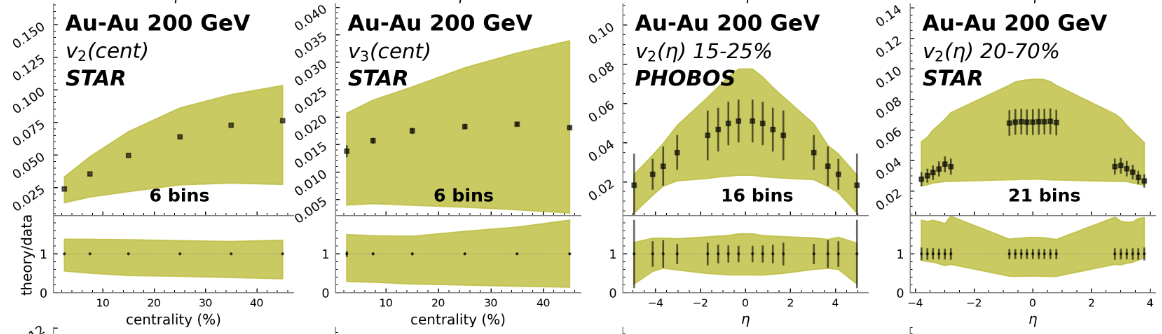
\includegraphics[width=.95\linewidth]{img/Au-Au-prior.png}

\vspace{0.15cm}

{\Large $\Downarrow$}

\small Bayesian calibration

\vspace{0.15cm}

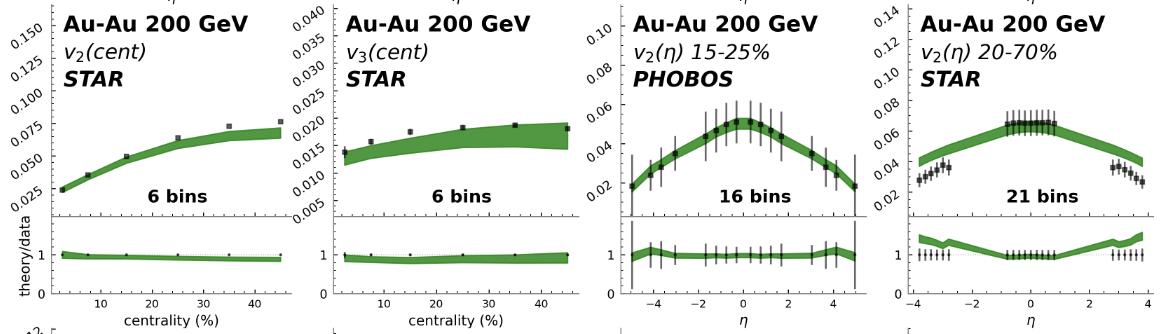
\includegraphics[width=.95\linewidth]{img/Au-Au-posterior.png}

\end{columns}

\vspace{0.4cm}
\small
Changing $\Sigma_{\rm sys}$ modifies the likelihood and therefore the posterior constraints.

\end{frame}
%--------------------------------------------------------
\section{Universal Scaled Spectra}

\begin{frame}
\frametitle{Universal Scaled Spectra}

\begin{columns}[T]

%====================================================
% LEFT
%====================================================

\column{0.48\textwidth}

\centering
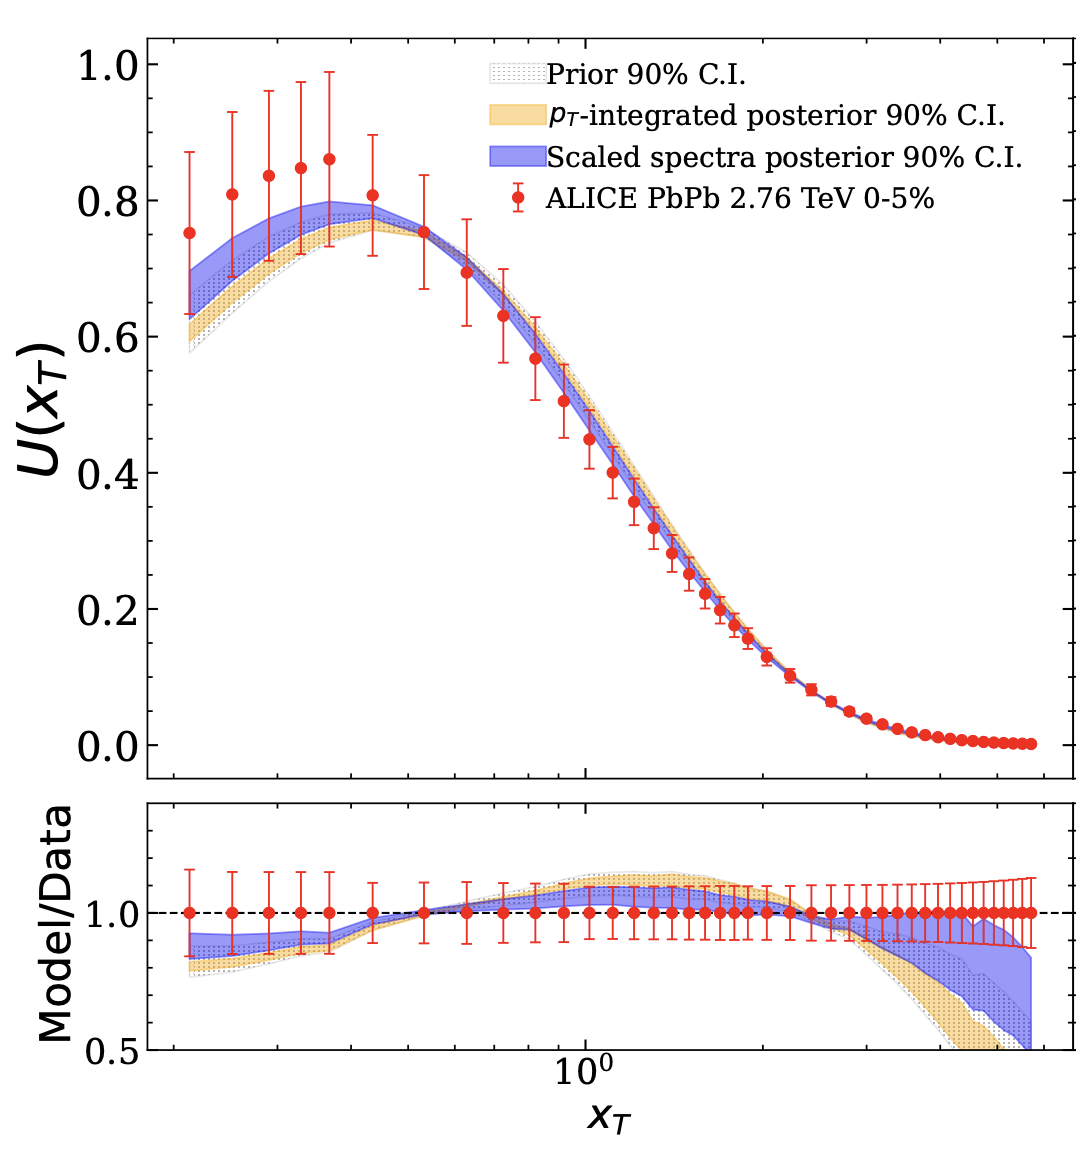
\includegraphics[width=\linewidth]{img/universal_scaled_spectra.png}

\vspace{0.1cm}

\tiny
Identified-particle spectra collapse onto a universal curve after rescaling.
{\tiny
Domingues \& Luzum, arXiv:2603.15891 (2026).
}
%====================================================
% RIGHT
%====================================================

\column{0.52\textwidth}

\small

\textbf{Motivation}

\begin{itemize}
    \item Remove trivial dependence on particle yield.
    \item Remove the characteristic momentum scale.
    \item Compare only the \textbf{shape} of the spectra.
\end{itemize}

\vspace{0.2cm}

The transverse momentum is rescaled as

\[
x_T=\frac{p_T}{\langle p_T\rangle},
\]

and the corresponding scaled spectrum is

\[
U(x_T)
=
\frac{\langle p_T\rangle}{N}
\frac{dN}{dp_T}
=
\frac{1}{N}
\frac{dN}{dx_T}.
\]
\end{columns}

\scriptsize
After this normalization, spectra from different collision centralities become nearly universal.



\end{frame}

%--------------------------------------------------------


\begin{frame}
\frametitle{Bayesian Calibration using Universal Scaled Spectra}

\begin{columns}[T]

%====================================================
% LEFT
%====================================================

\column{0.48\textwidth}

\centering

\Large

\[
\boxed{
\text{Universal Scaled Spectra}
}
\]

\vspace{0.25cm}

\[
\Downarrow
\]

\vspace{0.15cm}

\[
\boxed{
\text{Hydrodynamic Model}
}
\]

\vspace{0.25cm}

\[
\Downarrow
\]

\vspace{0.15cm}

\[
\boxed{
\text{Gaussian Process Emulator}
}
\]

\vspace{0.25cm}

\[
\Downarrow
\]

\vspace{0.15cm}

\[
\boxed{
\text{Bayesian Inference}
}
\]

%====================================================
% RIGHT
%====================================================

\column{0.52\textwidth}

\small

\textbf{Calibration procedure}

\begin{itemize}
    \item Universal scaled spectra are used as experimental observables.
    \item Event-by-event hydrodynamic simulations are replaced by Gaussian Process emulators.
    \item Bayesian inference constrains the QGP model parameters.
\end{itemize}

\vspace{0.25cm}

\textbf{This work}

\begin{itemize}
    \item Keep the original Bayesian calibration framework.
    \item Replace the diagonal experimental covariance matrix by correlated covariance models (CS and RBF).
    \item Quantify the impact on the inferred QGP parameters.
\end{itemize}

\end{columns}

\end{frame}
% \section{Preliminary Results}

%--------------------------------------------------------

\begin{frame}
\frametitle{Preliminary Results}

\centering
\scriptsize
ALICE Pb--Pb $\sqrt{s_{NN}}=2.76$ TeV

HEPData: \texttt{ins1222333}

\vspace{0.15cm}

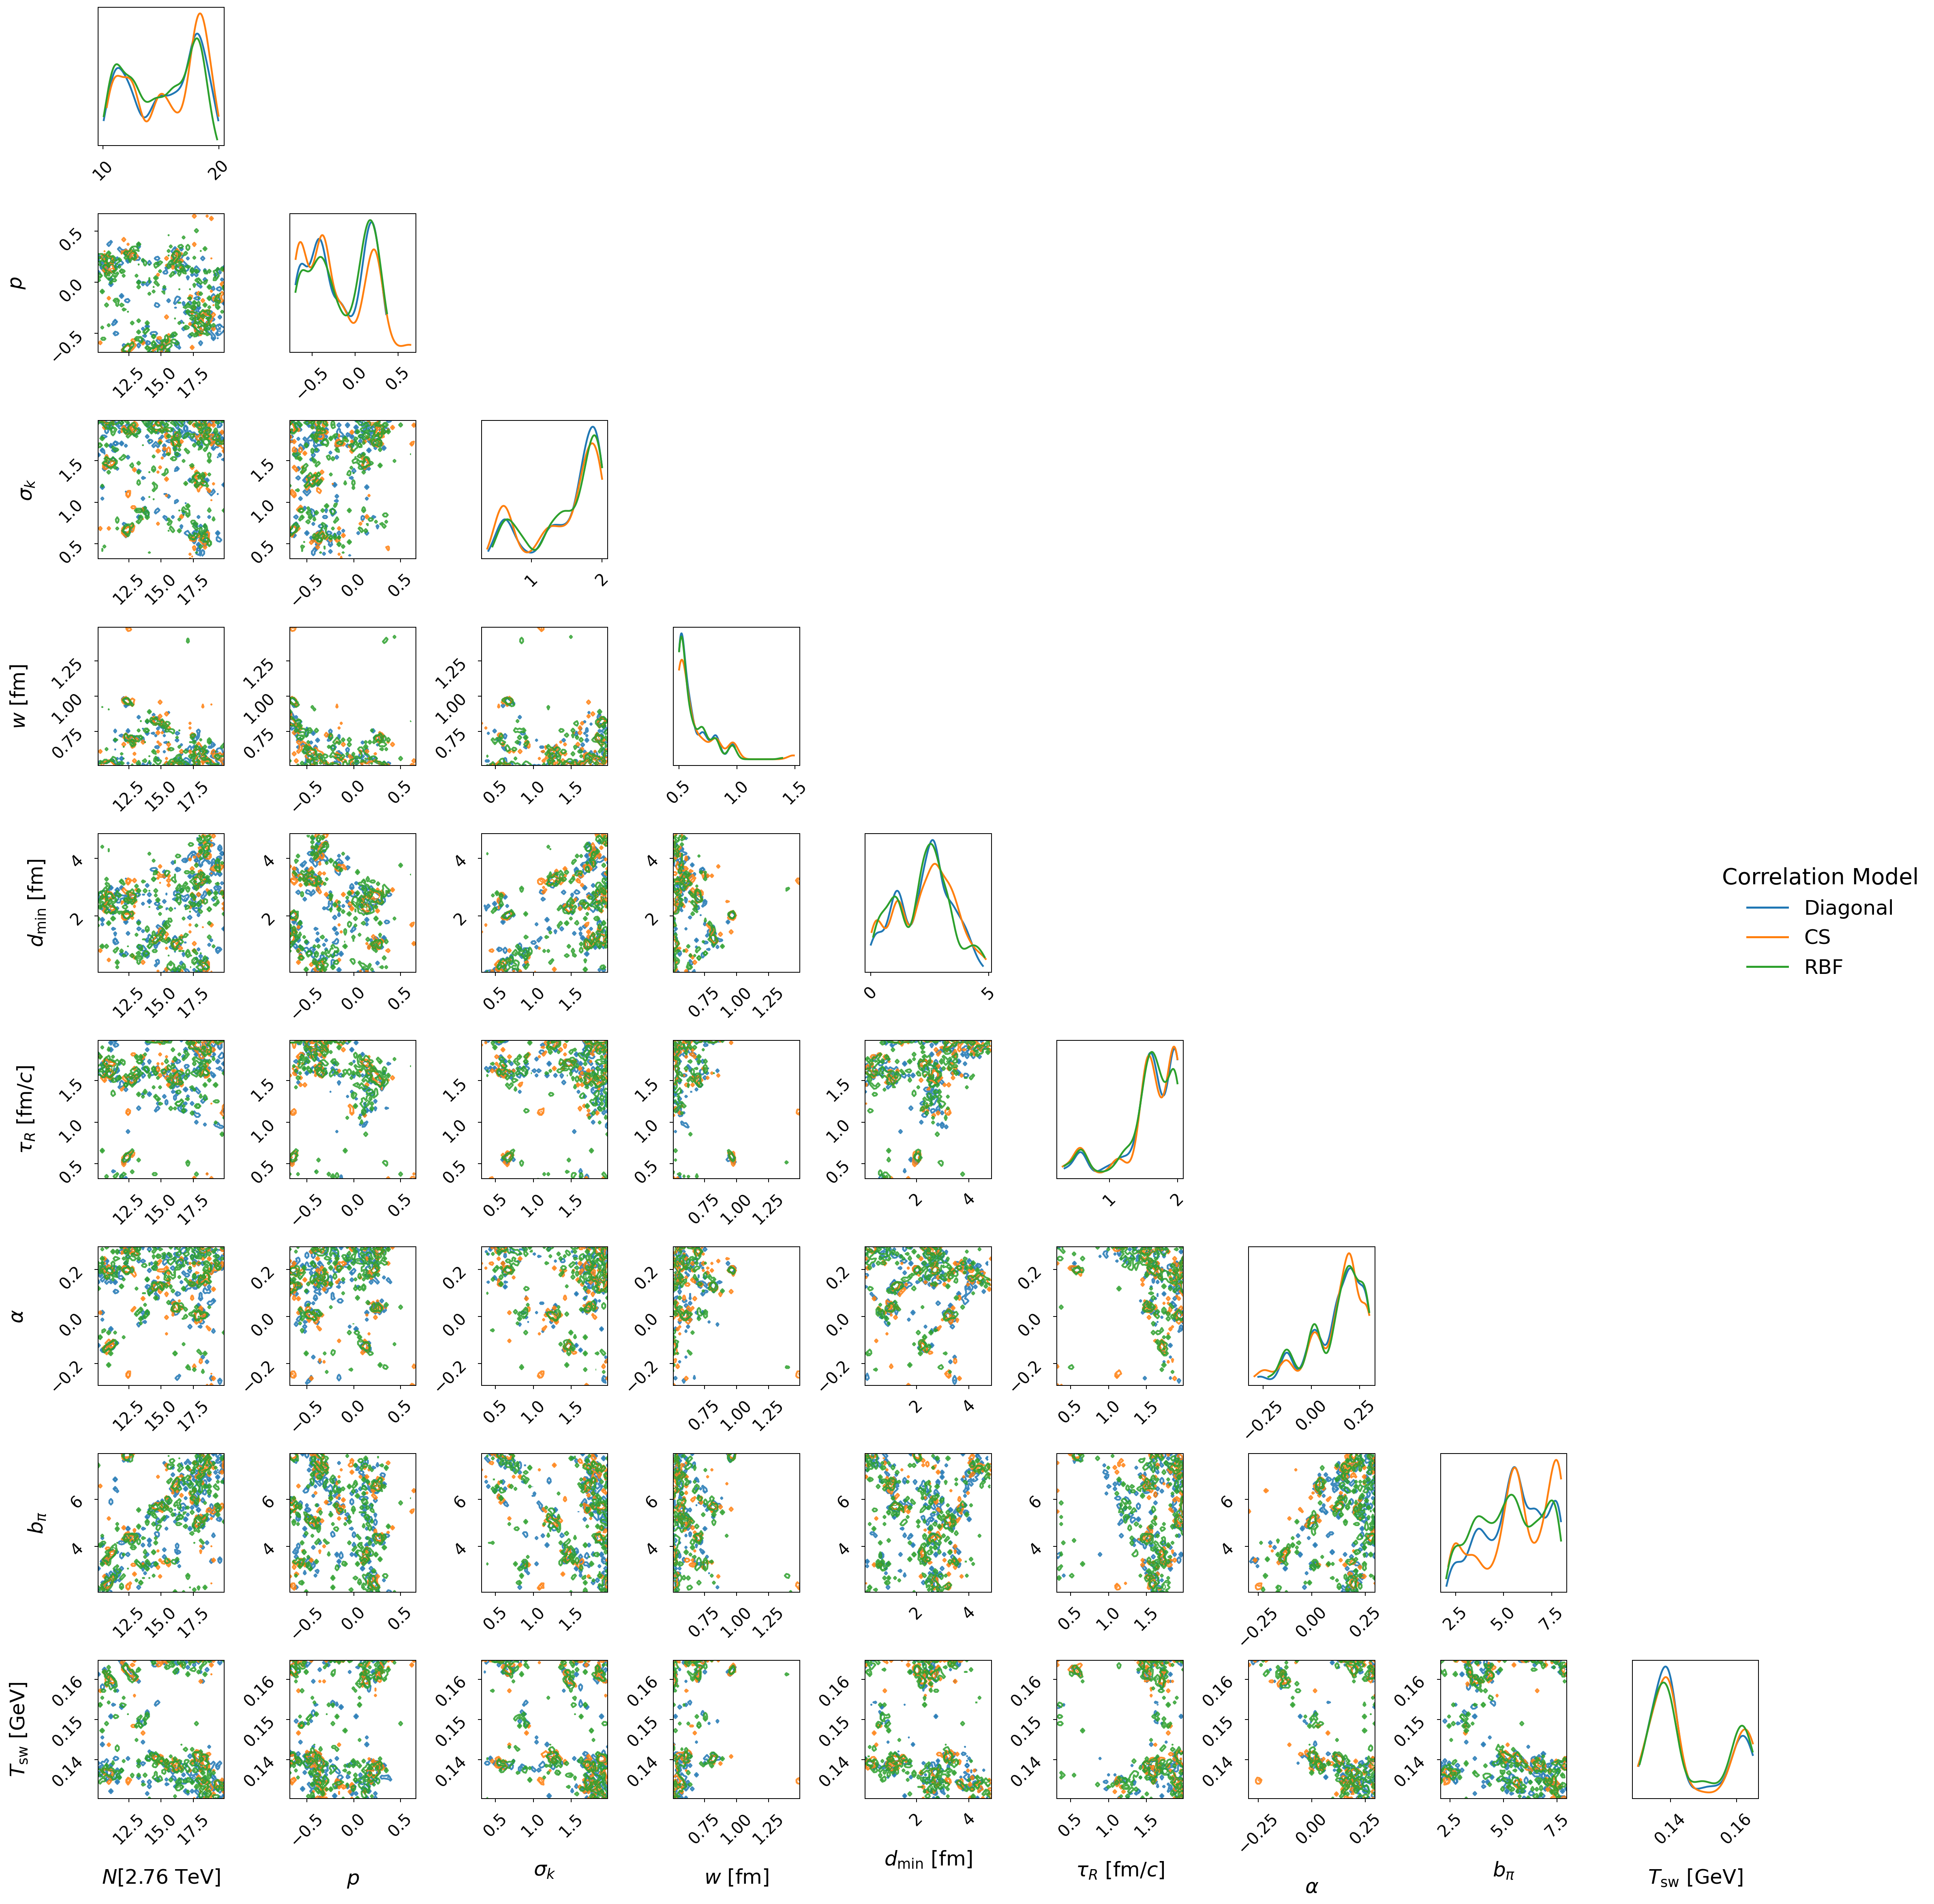
\includegraphics[width=0.48\textwidth]{img/corner_all_models_1.png}
\hfill
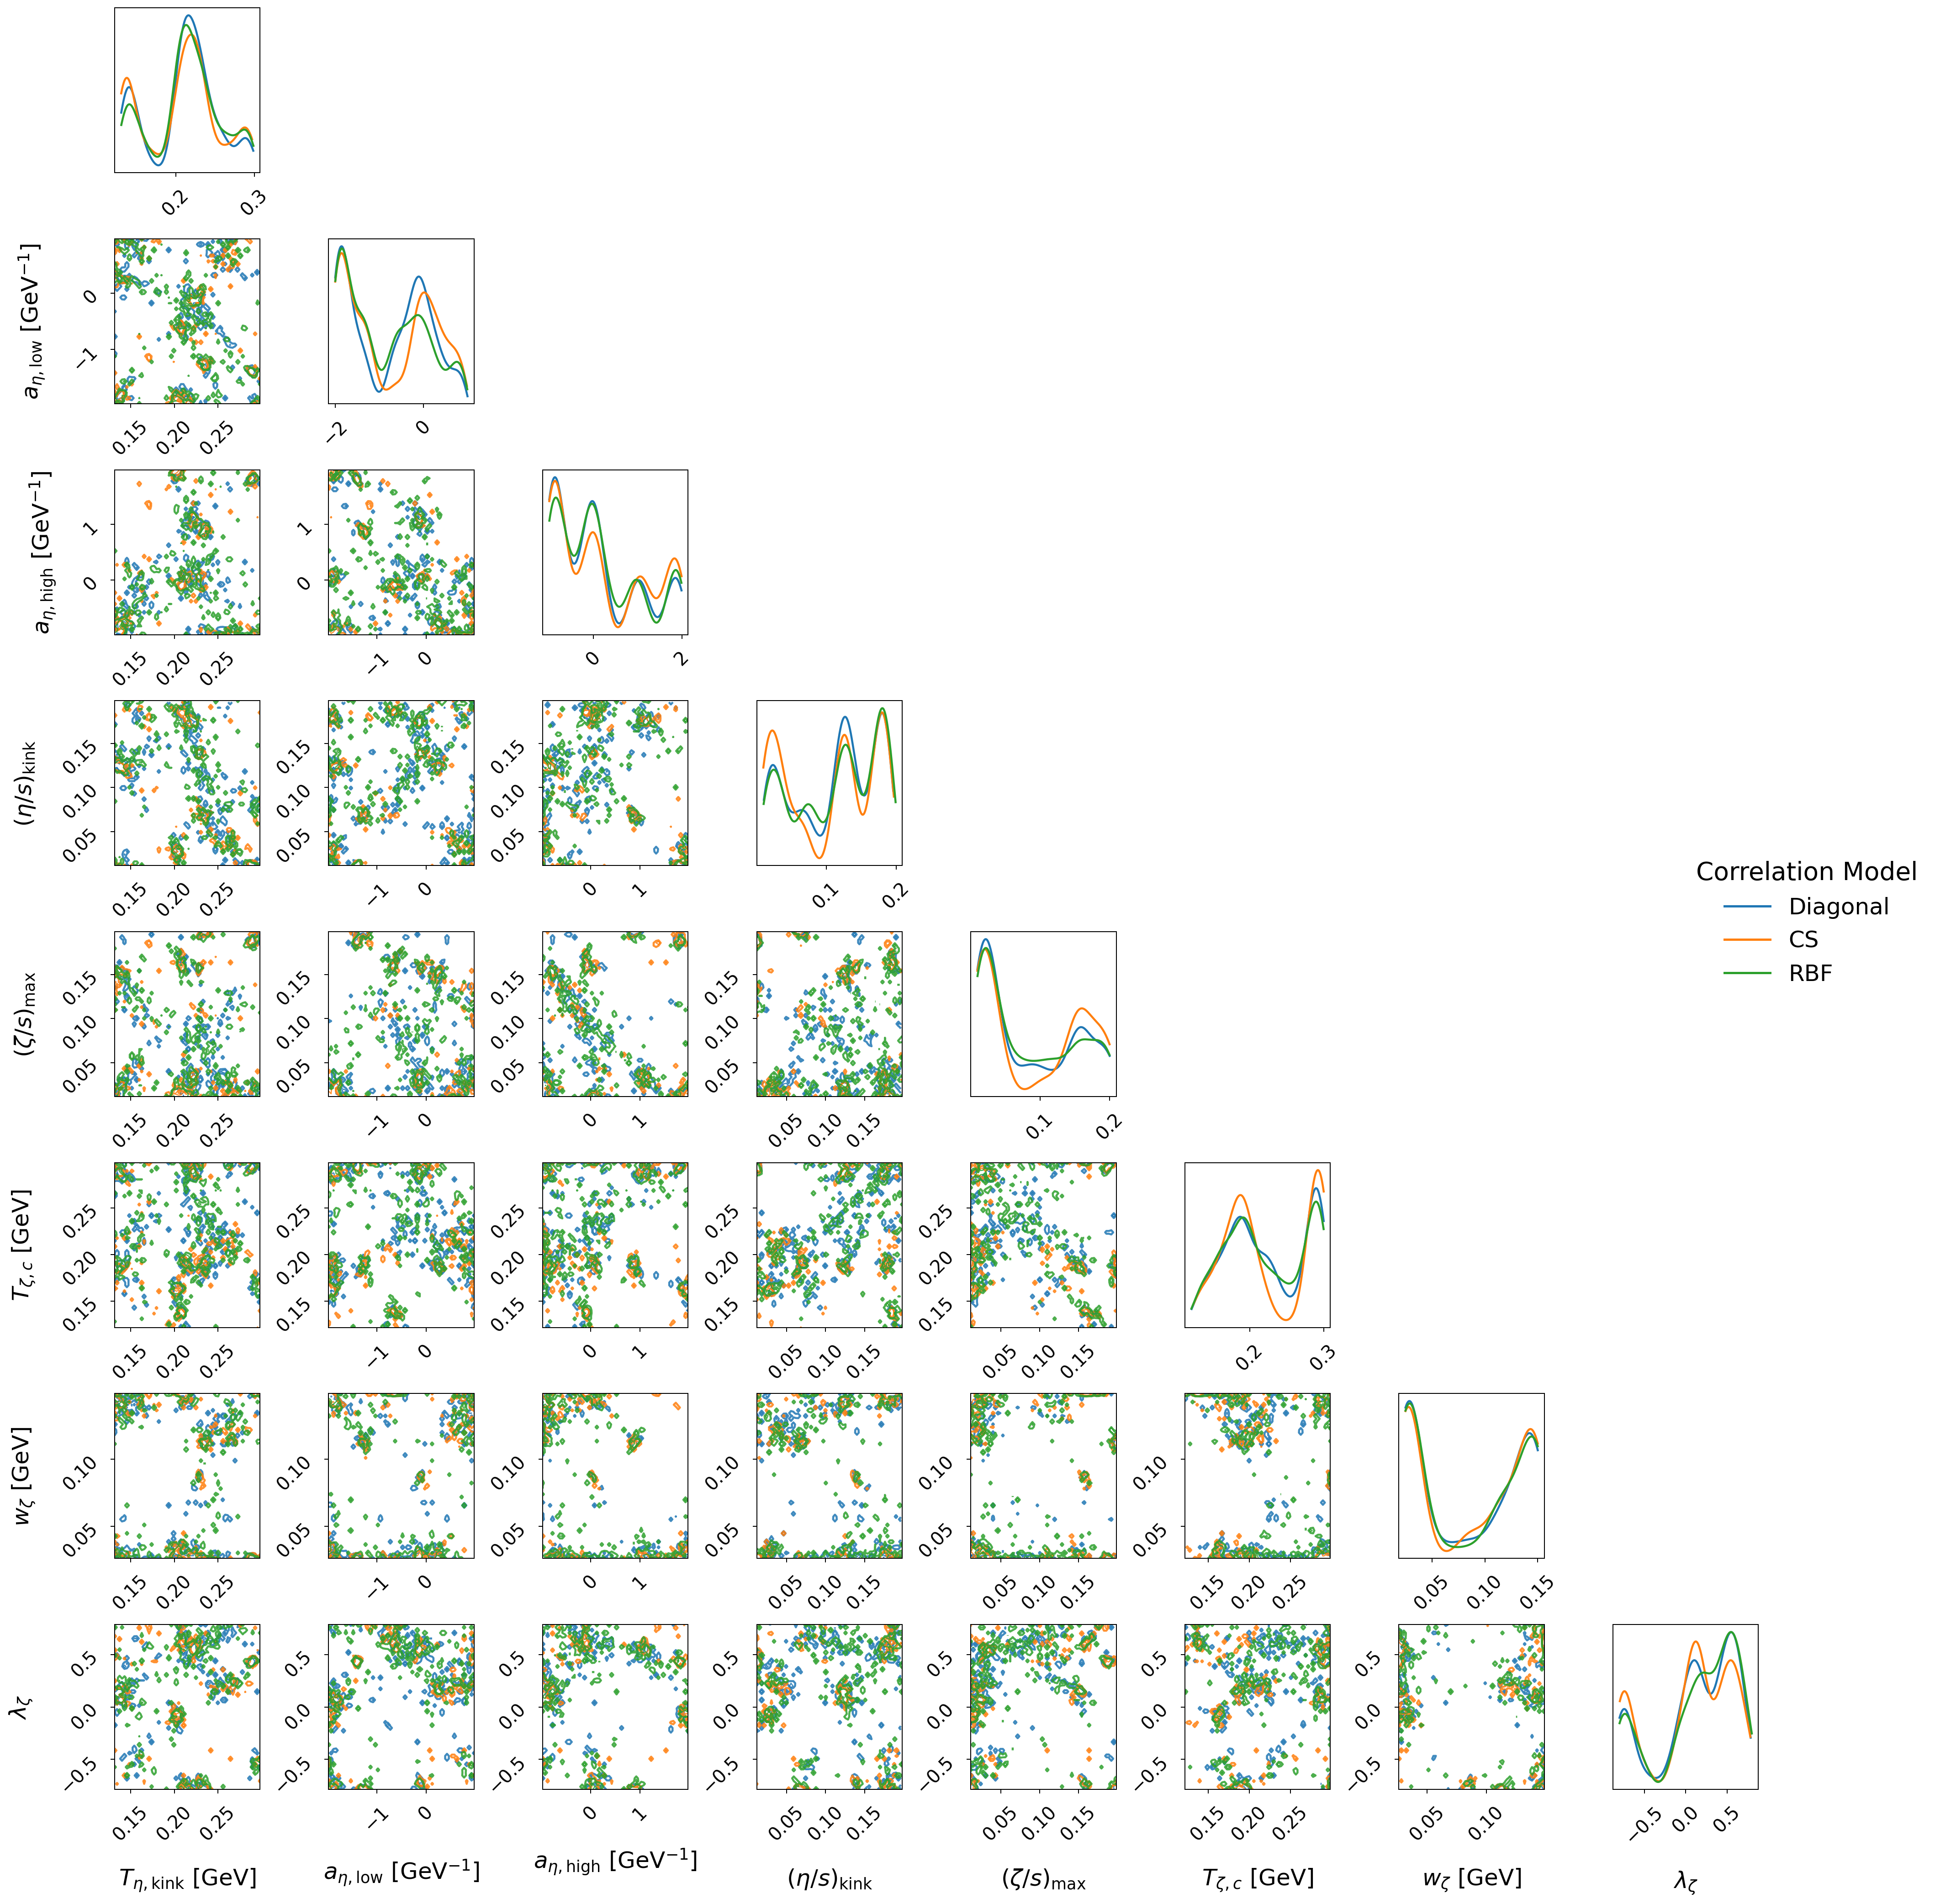
\includegraphics[width=0.48\textwidth]{img/corner_all_models_2.png}


\tiny
Posterior distributions using diagonal, compound-symmetry (CS), and RBF covariance models.

\end{frame}

%--------------------------------------------------------

% \begin{frame}
% \frametitle{Transport Parameter Constraints}

% \centering
% \scriptsize
% ALICE Pb--Pb $\sqrt{s_{NN}}=2.76$ TeV

% HEPData: \texttt{ins1222333}

% \vspace{0.15cm}

% 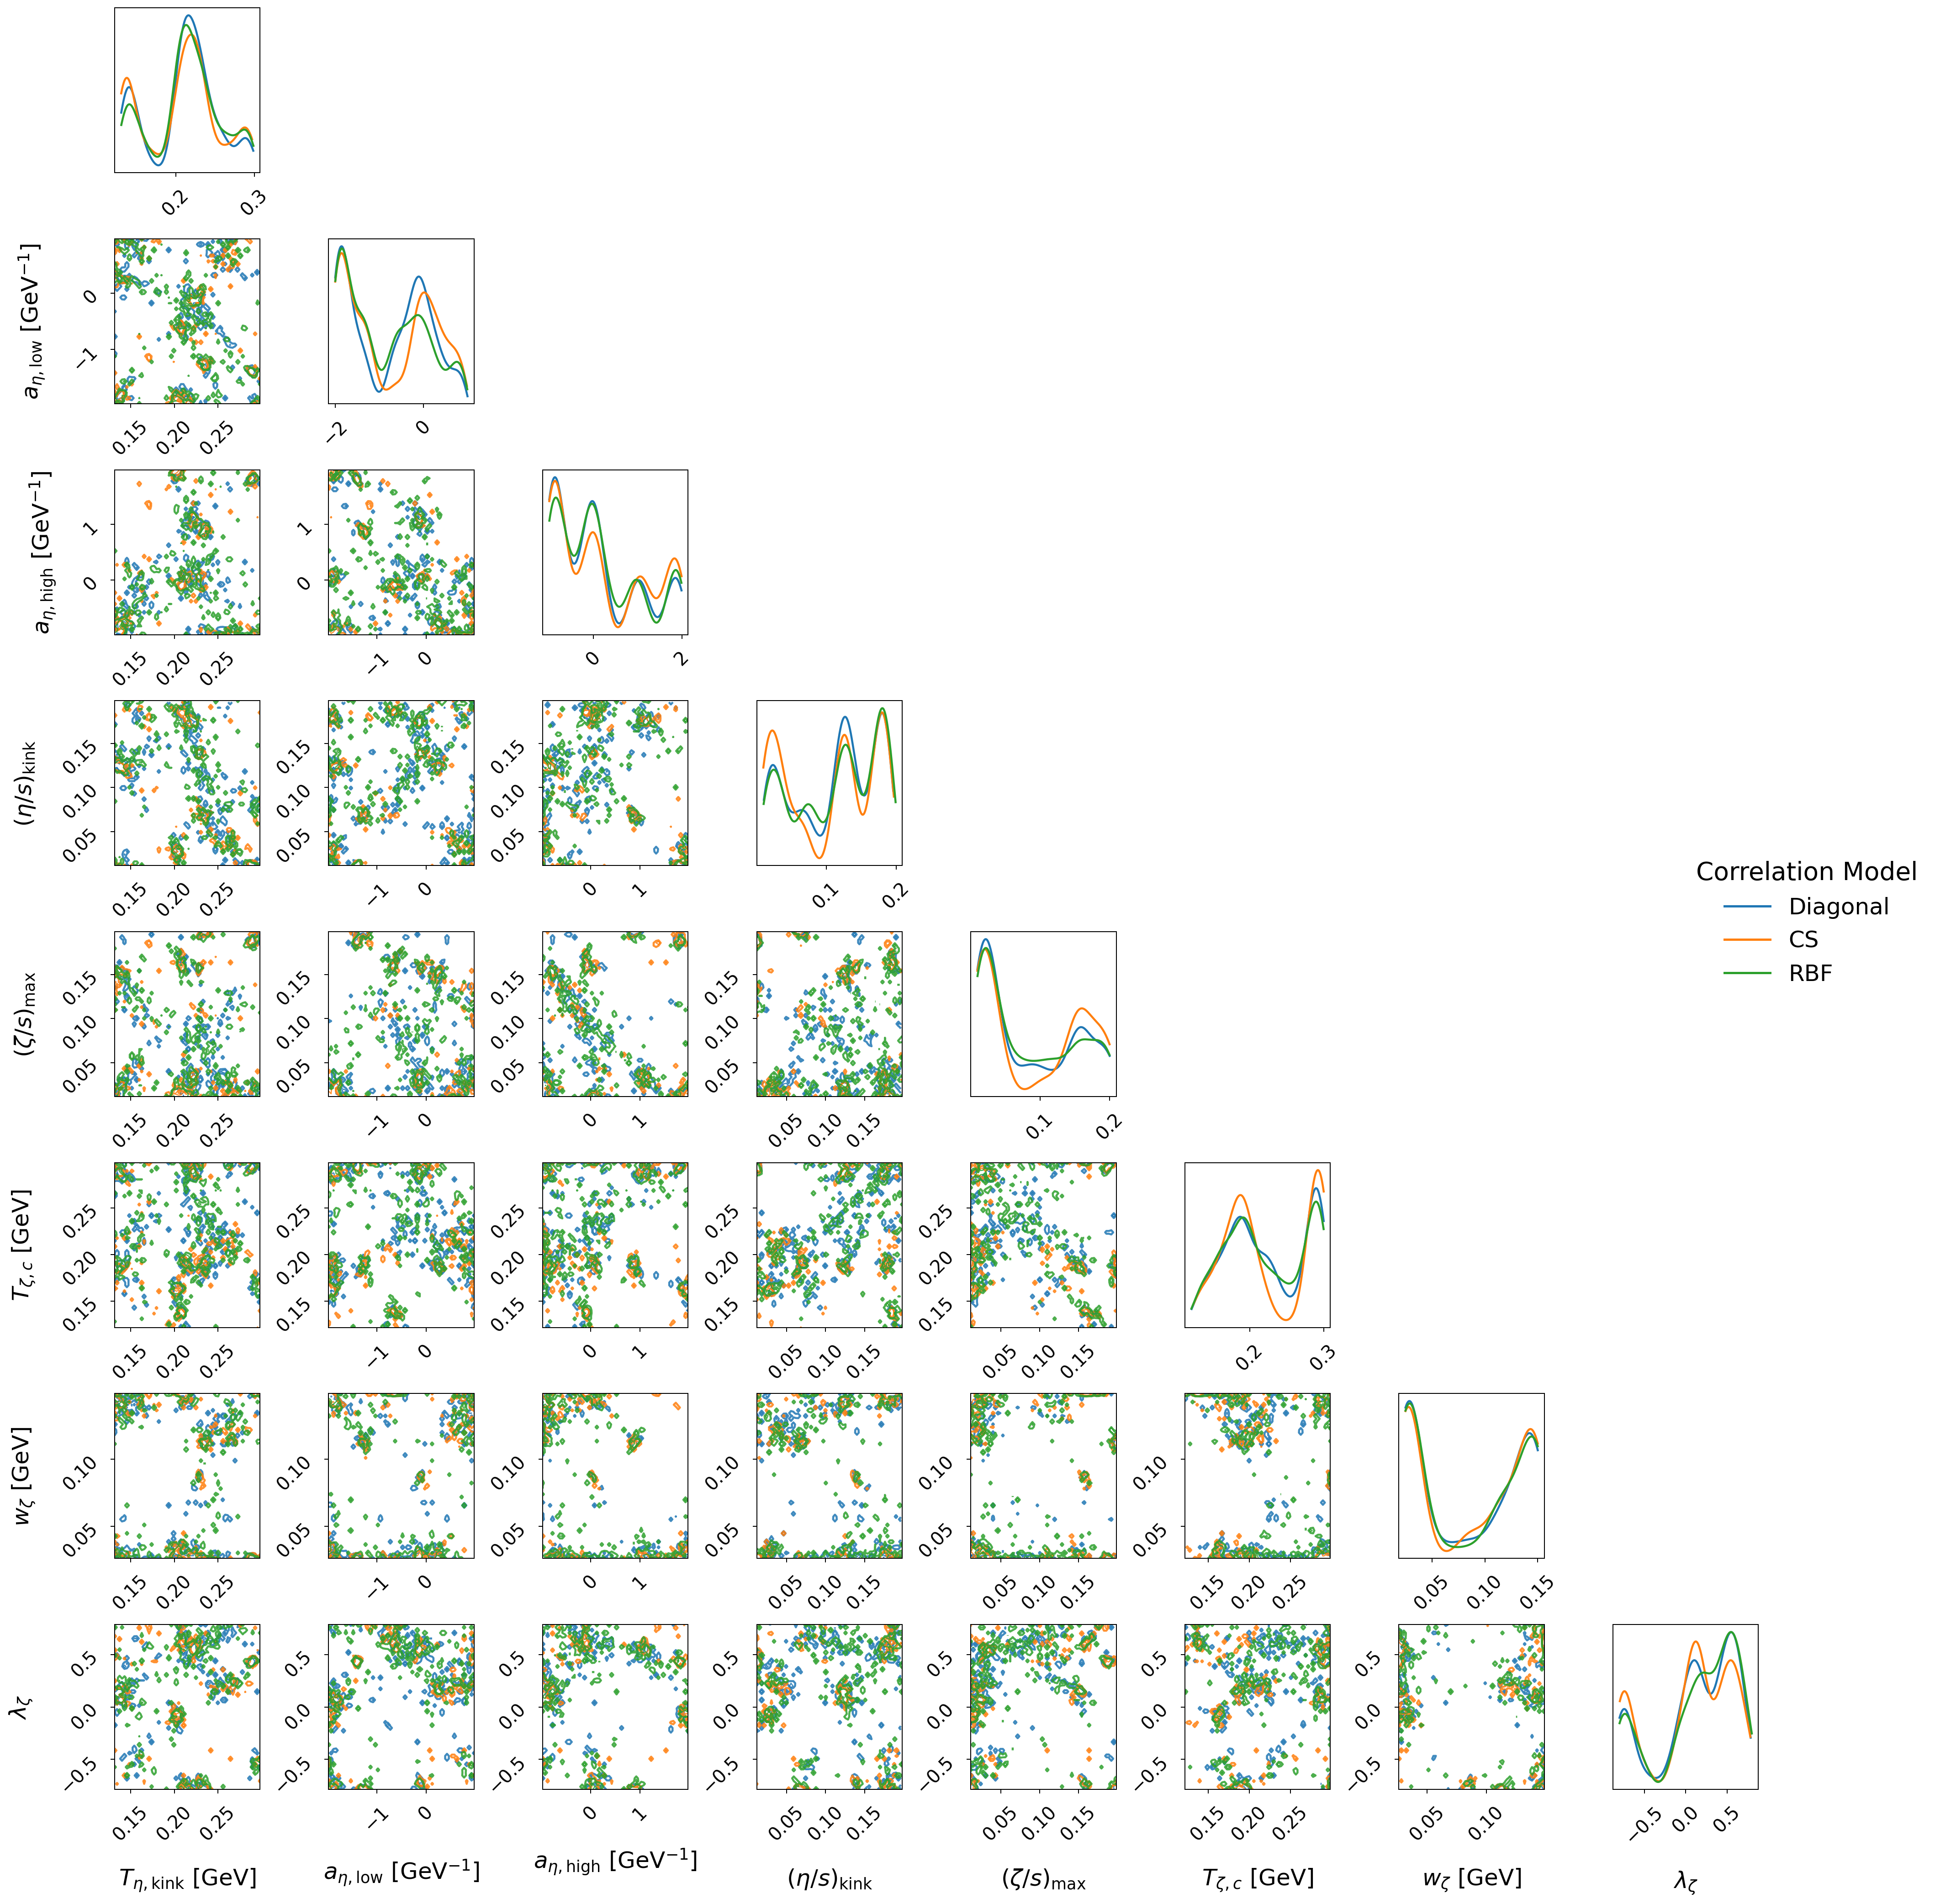
\includegraphics[width=0.48\textwidth]{img/corner_all_models_2.png}
% \hfill
% 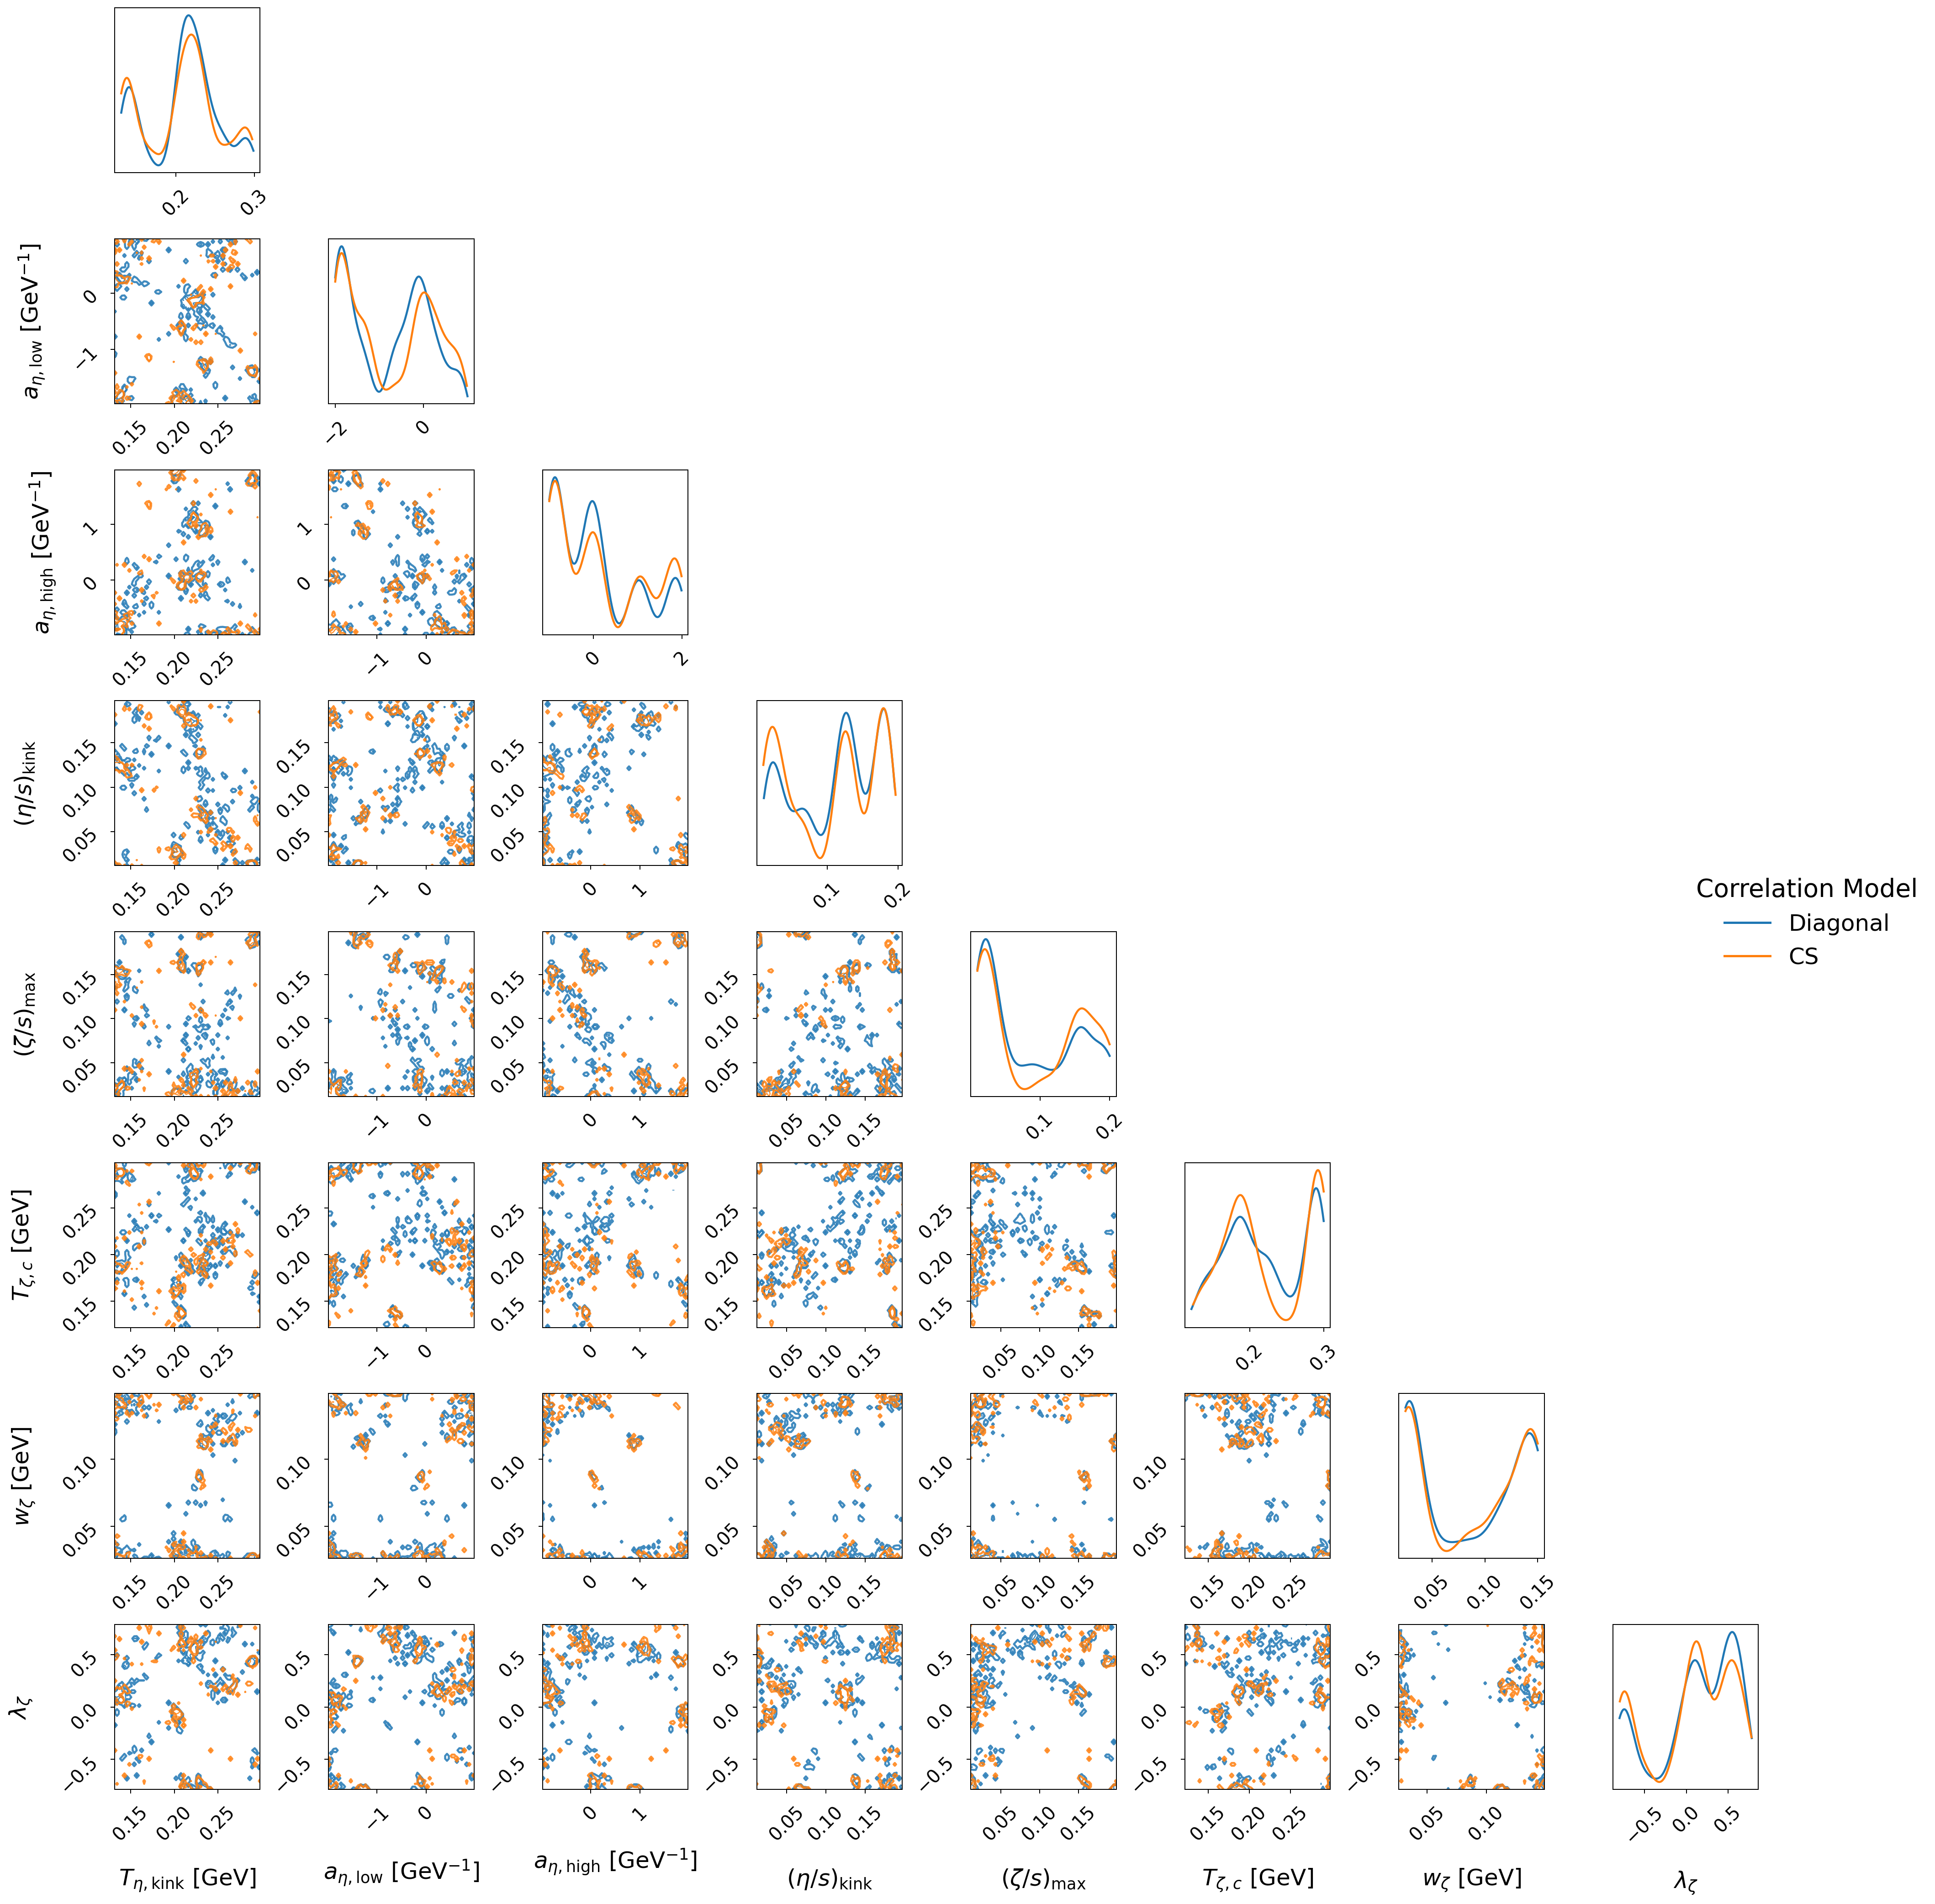
\includegraphics[width=0.48\textwidth]{img/corner_diag_vs_cs_2.png}

% \vspace{0.15cm}

% \tiny
% Left: posterior distributions using diagonal, compound-symmetry (CS), and RBF covariance models.
% Right: comparison between the diagonal and CS covariance models.

% \end{frame}

% %--------------------------------------------------------

% \begin{frame}
% \frametitle{Diagonal vs RBF: Initial-State Parameters}

% \centering
% \scriptsize
% ALICE Pb--Pb $\sqrt{s_{NN}}=2.76$ TeV

% HEPData: \texttt{ins1222333}

% \vspace{0.15cm}

% 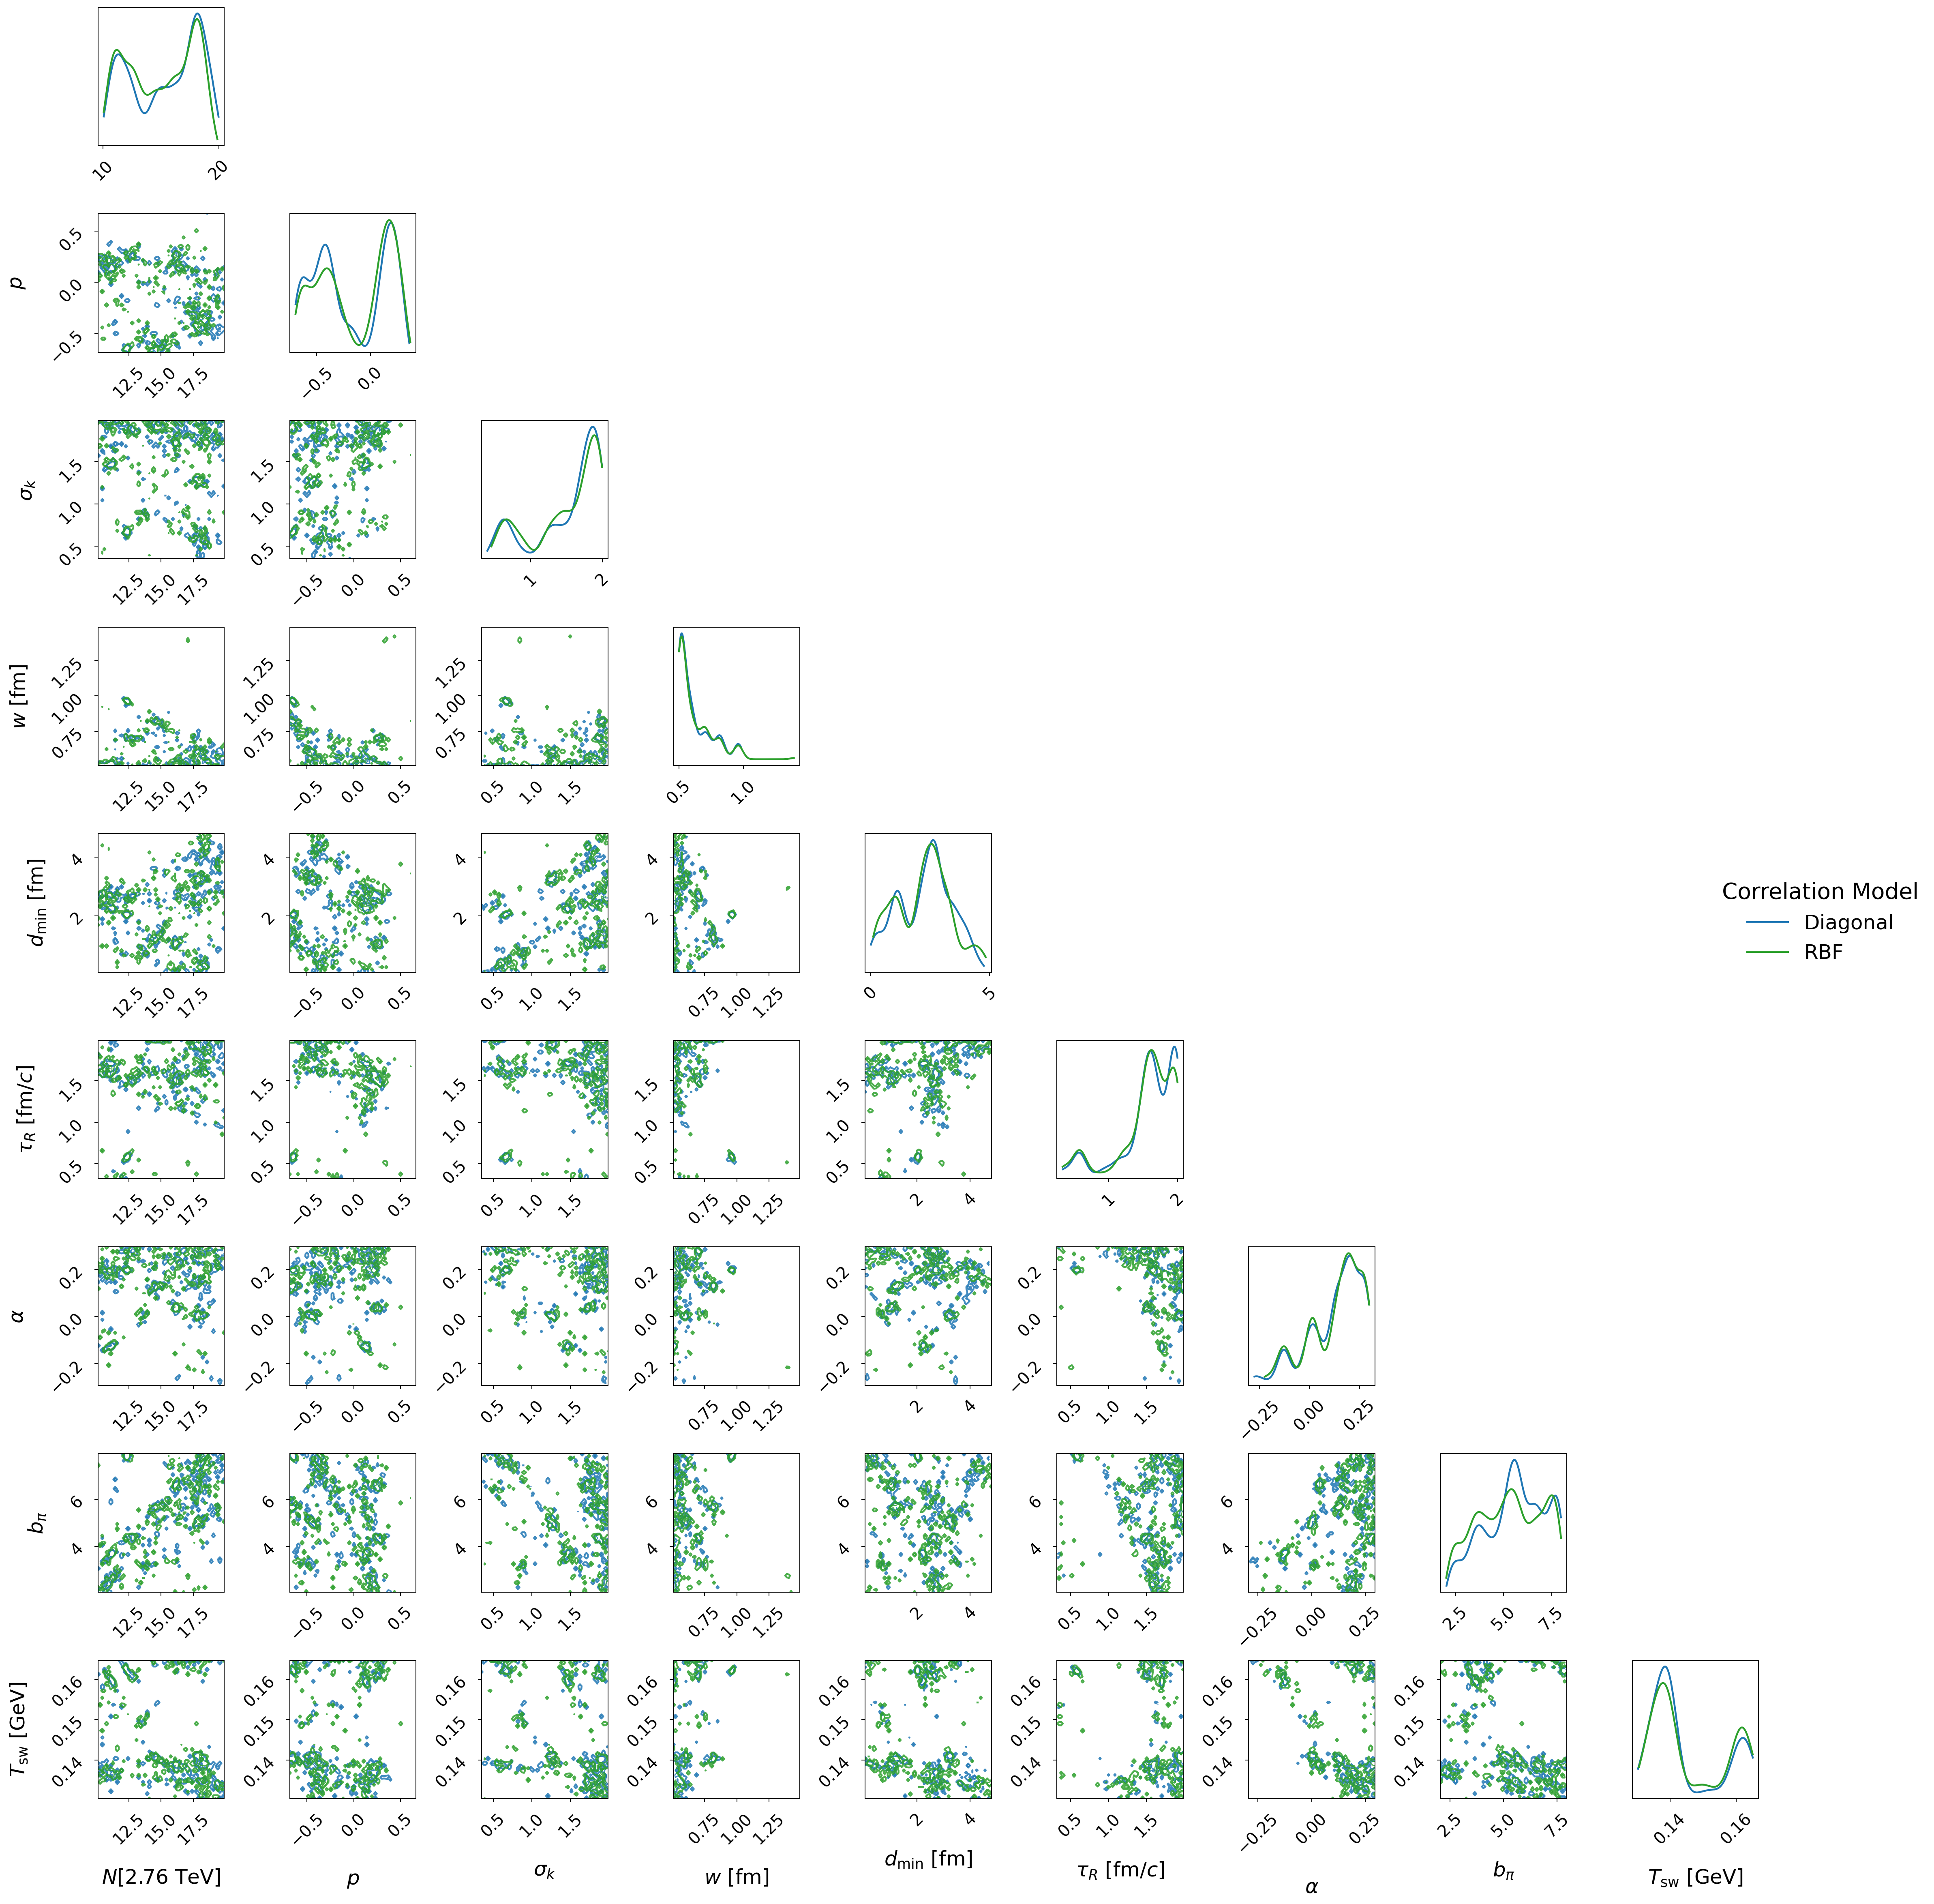
\includegraphics[width=0.82\textwidth]{img/corner_diag_vs_rbf_1.png}

% \vspace{0.15cm}

% \tiny
% Comparison between the diagonal and RBF experimental covariance models.

% \end{frame}

% %--------------------------------------------------------

% \begin{frame}
% \frametitle{Diagonal vs RBF: Transport Parameters}

% \centering
% \scriptsize
% ALICE Pb--Pb $\sqrt{s_{NN}}=2.76$ TeV

% HEPData: \texttt{ins1222333}

% \vspace{0.15cm}

% 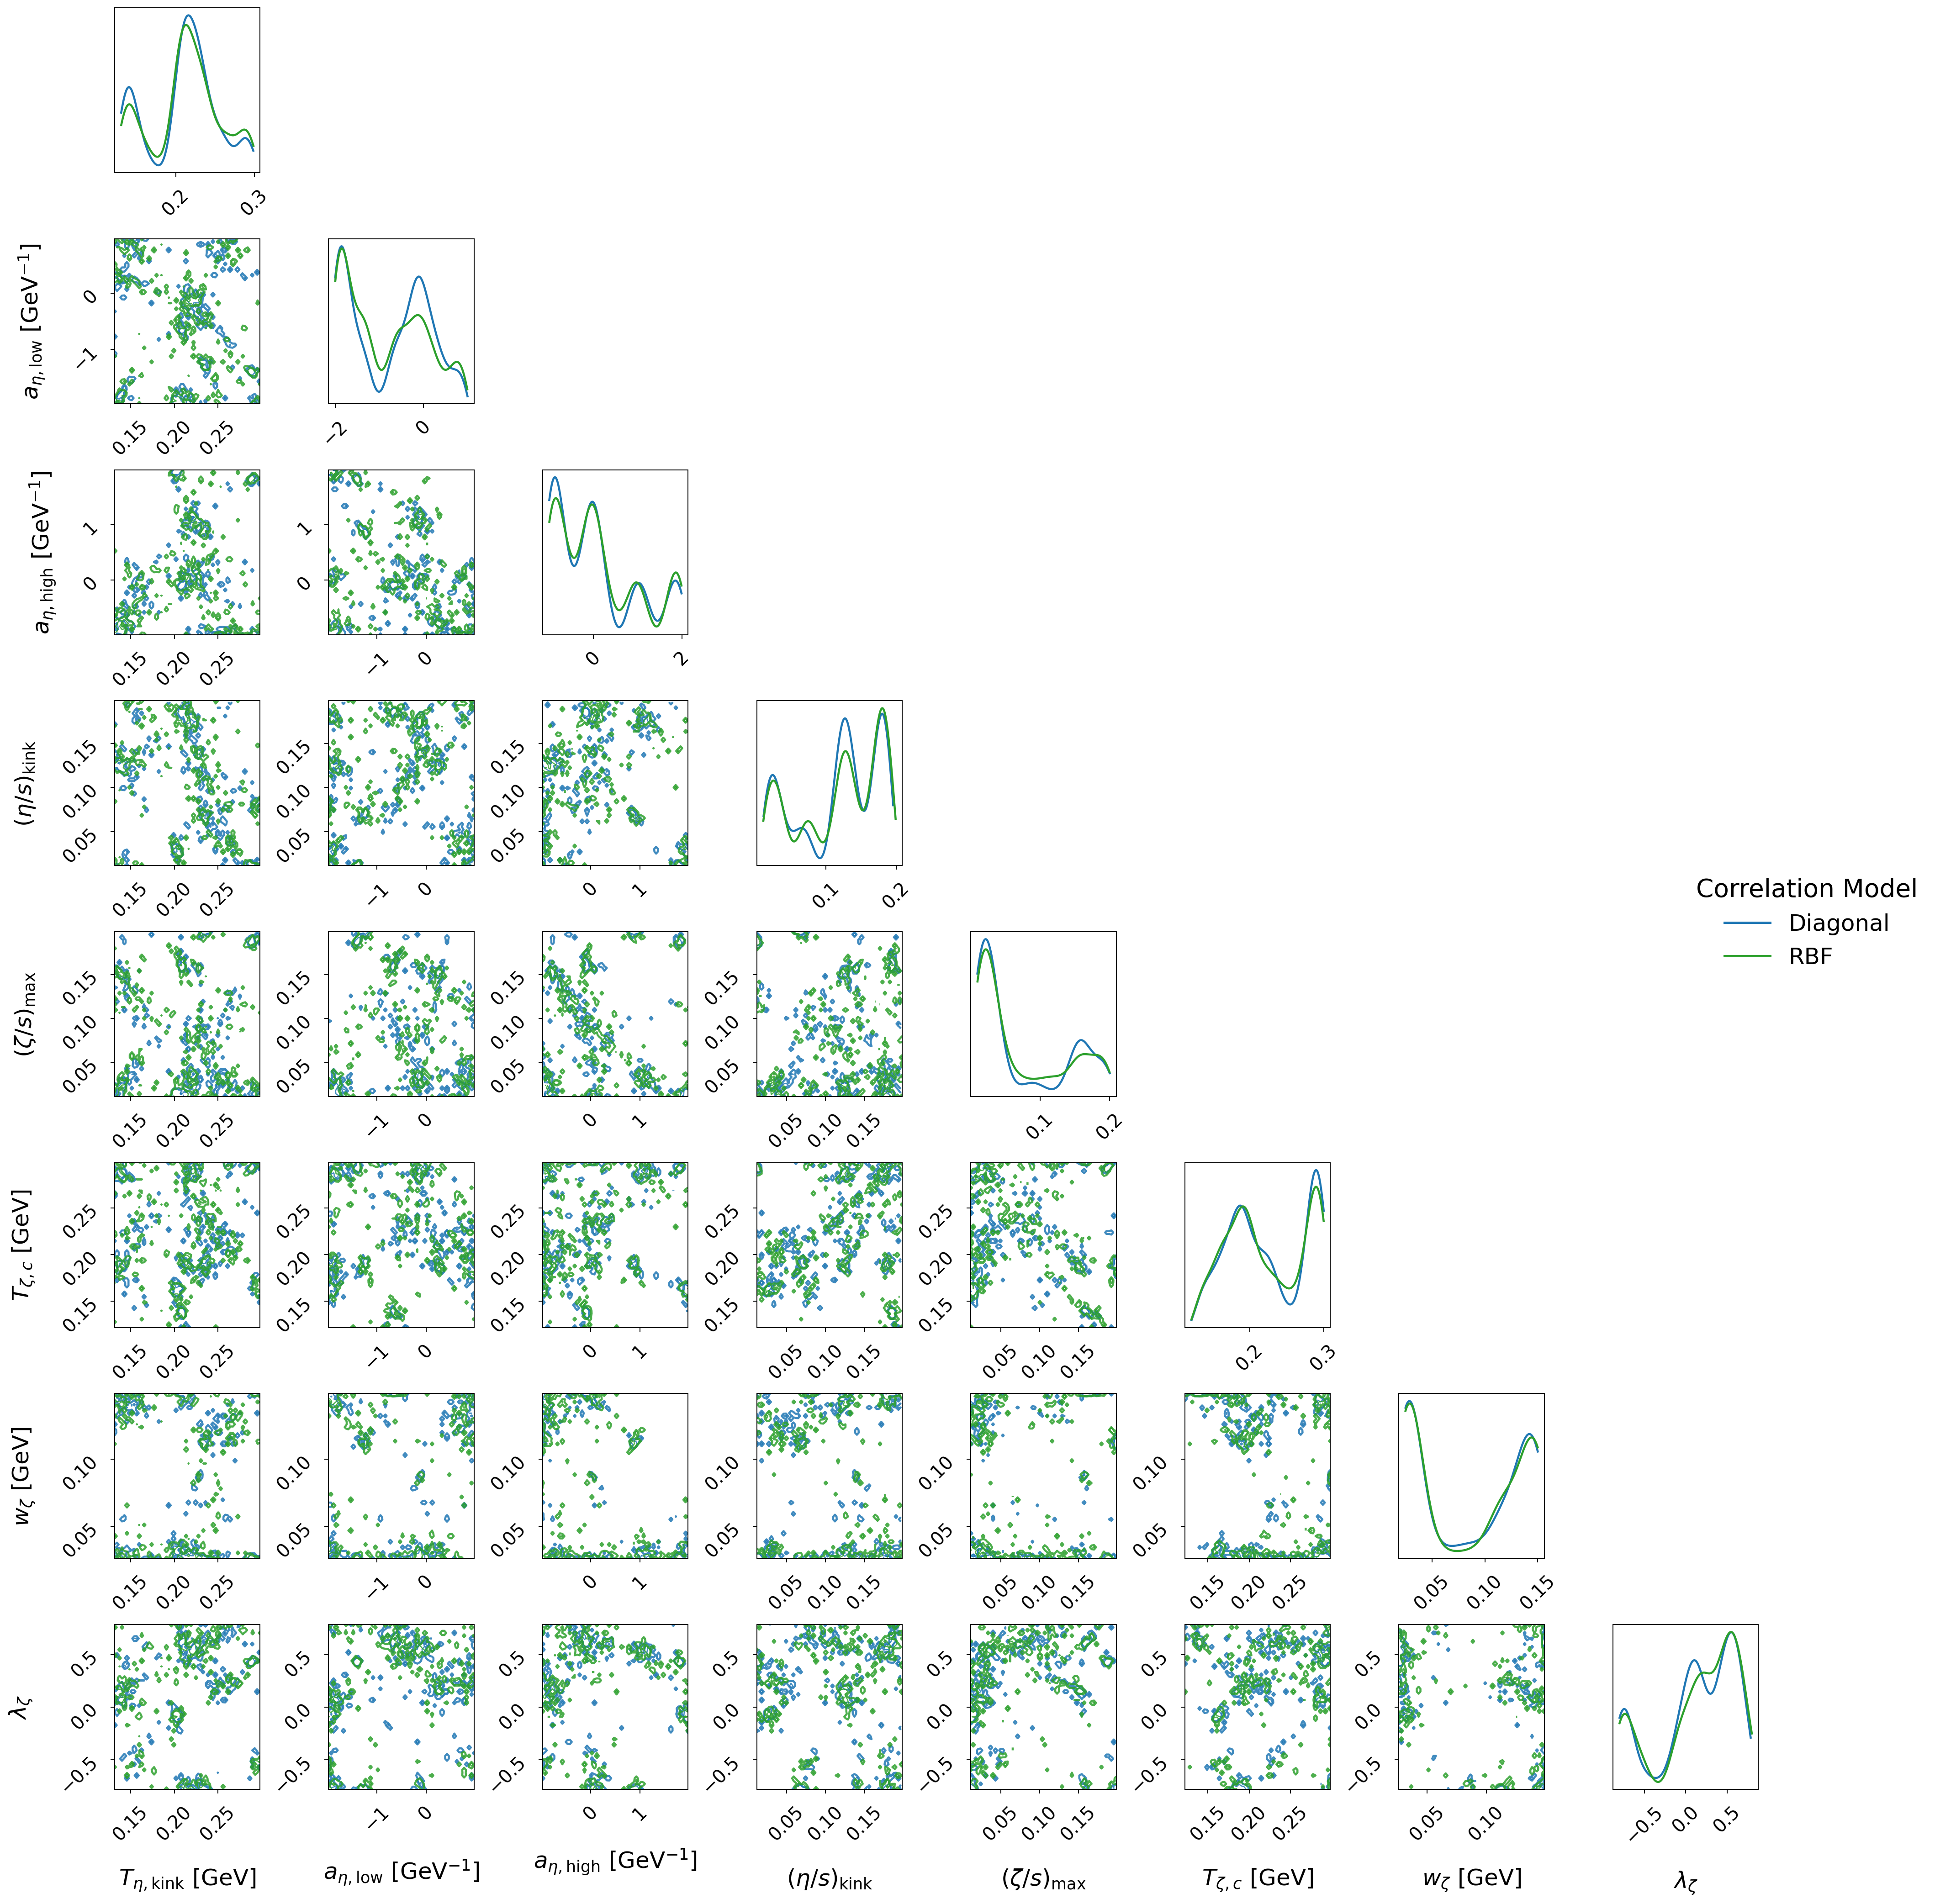
\includegraphics[width=0.82\textwidth]{img/corner_diag_vs_rbf_2.png}

% \vspace{0.15cm}

% \tiny
% Comparison between the diagonal and RBF experimental covariance models.

% \end{frame}
\section{Preliminary Results}

%--------------------------------------------------------

\begin{frame}
\frametitle{Preliminary Results}

\centering
\scriptsize
ALICE Pb--Pb $\sqrt{s_{NN}}=2.76$ TeV, universal spectra calibration

HEPData: \texttt{ins1222333}

\vspace{0.15cm}

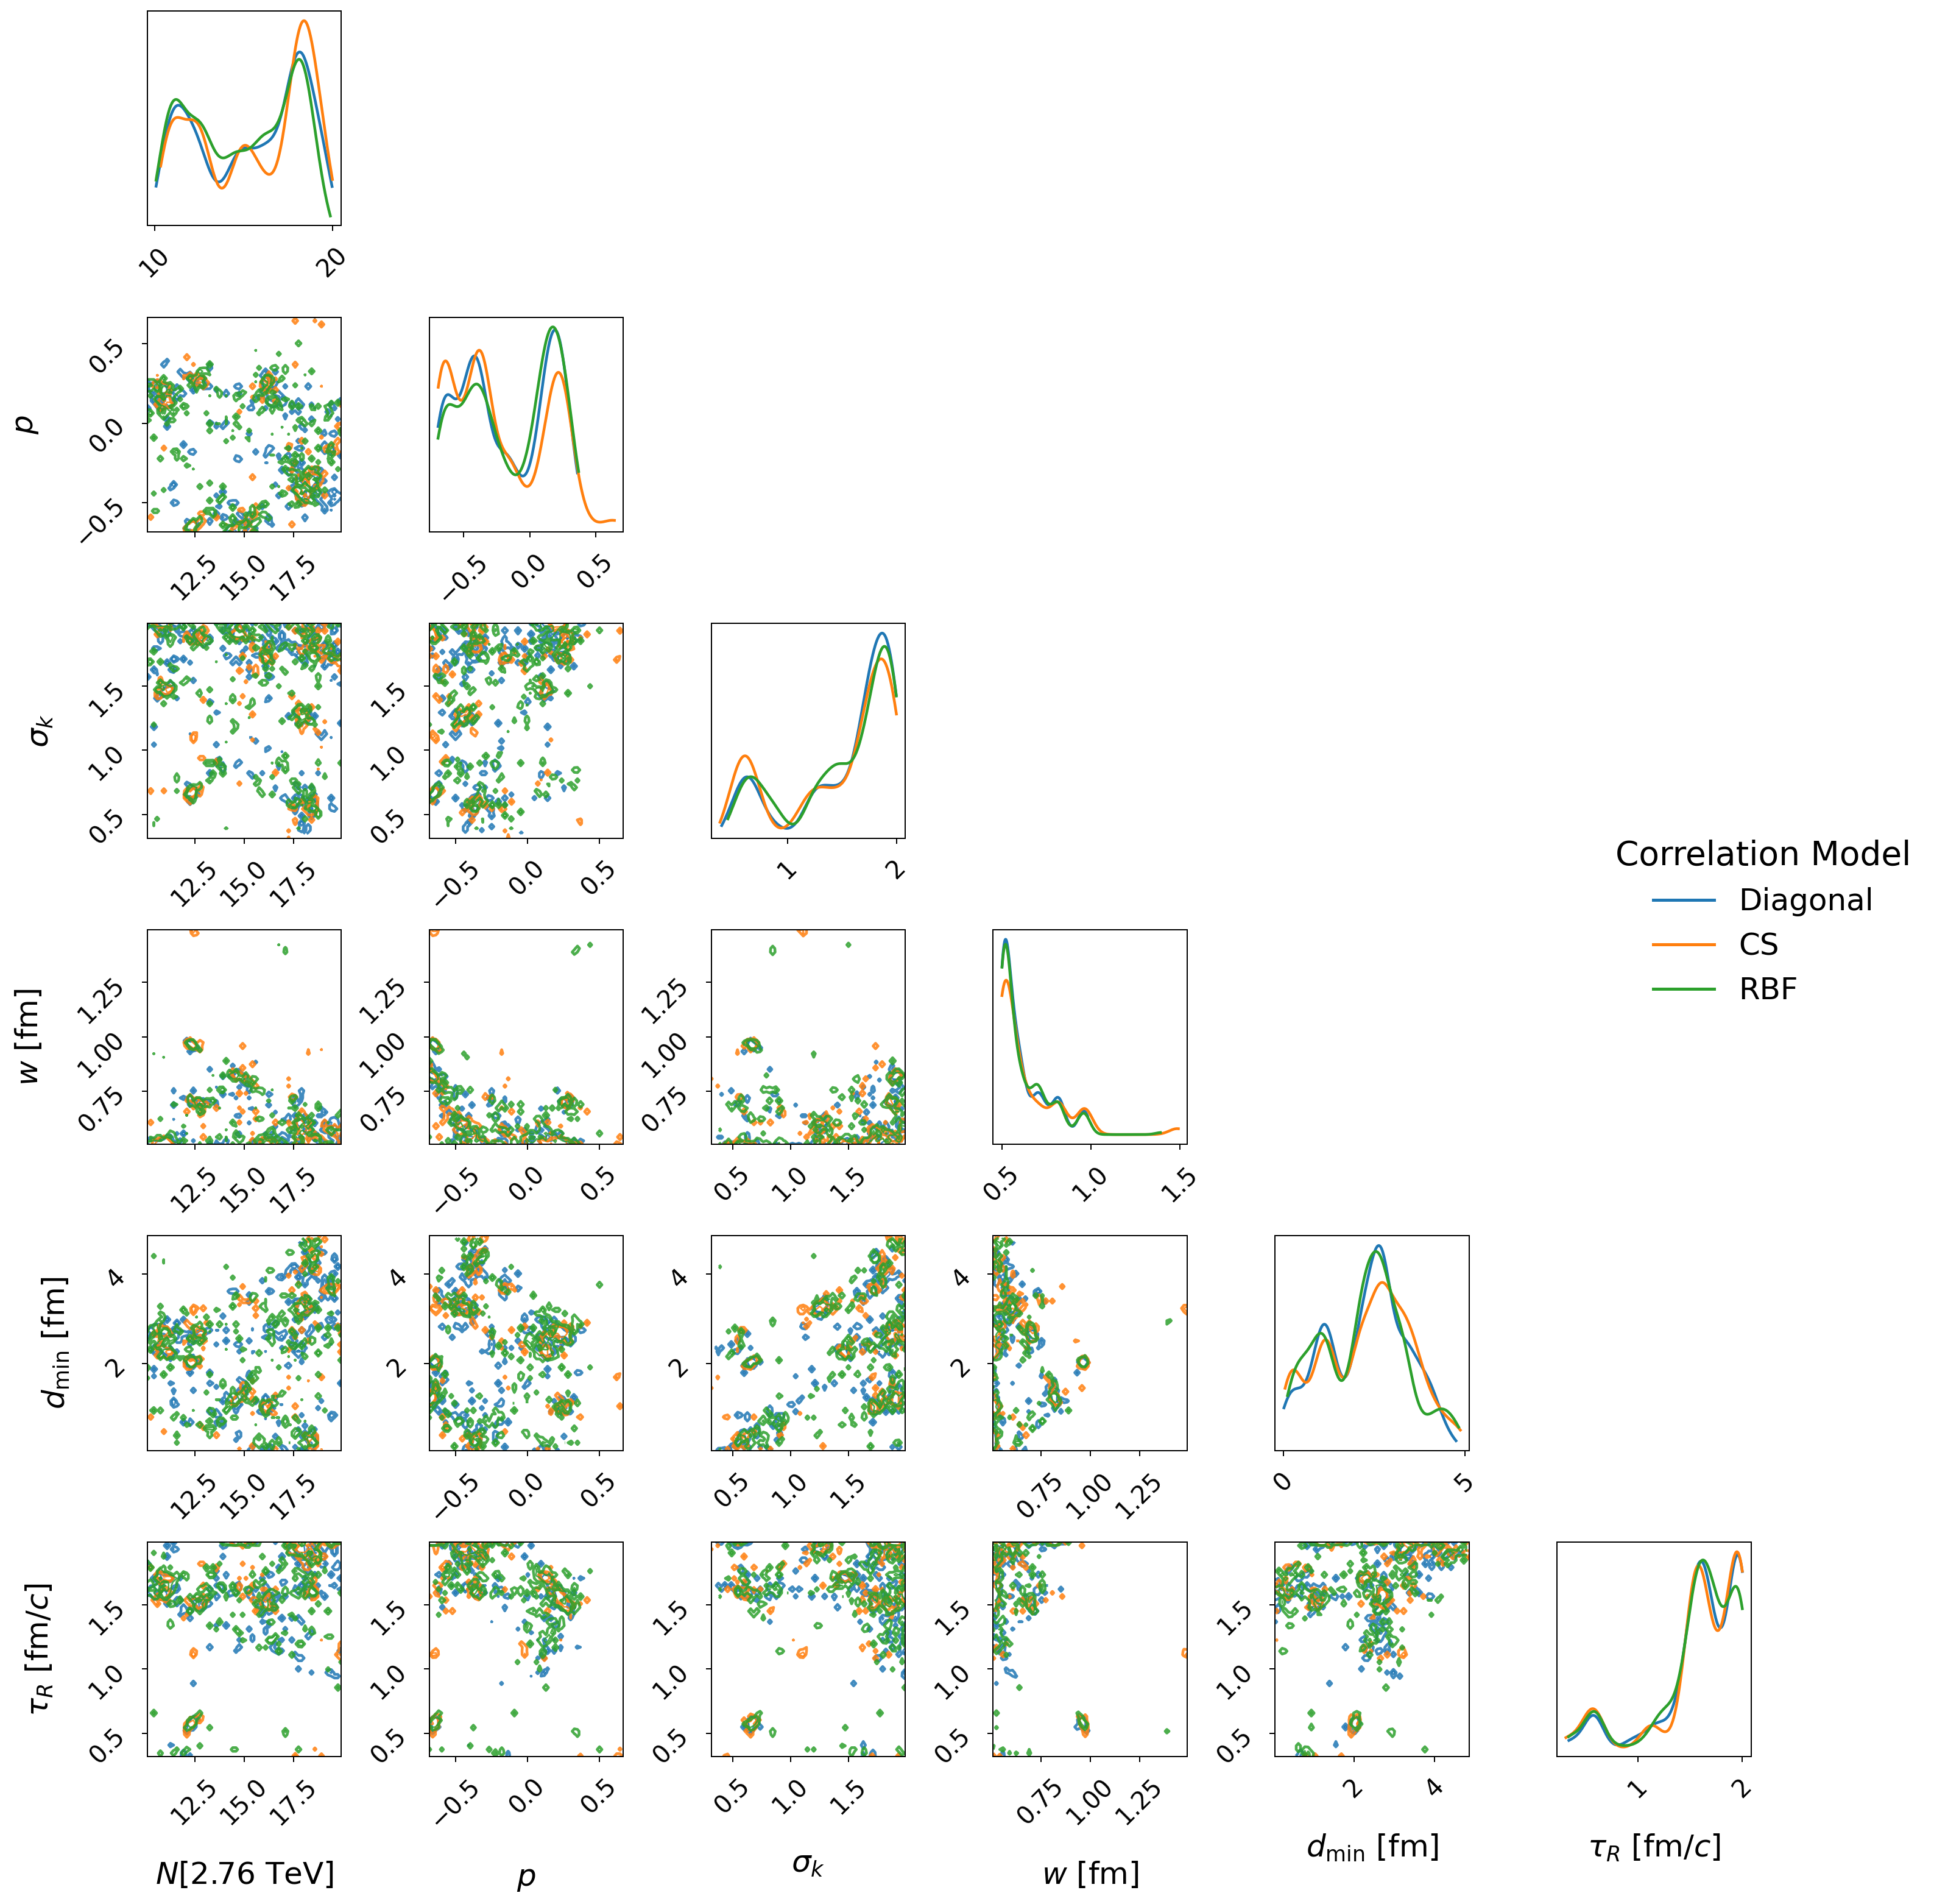
\includegraphics[width=0.48\textwidth]{img/corner_all_models_1-menos.png}
\hfill
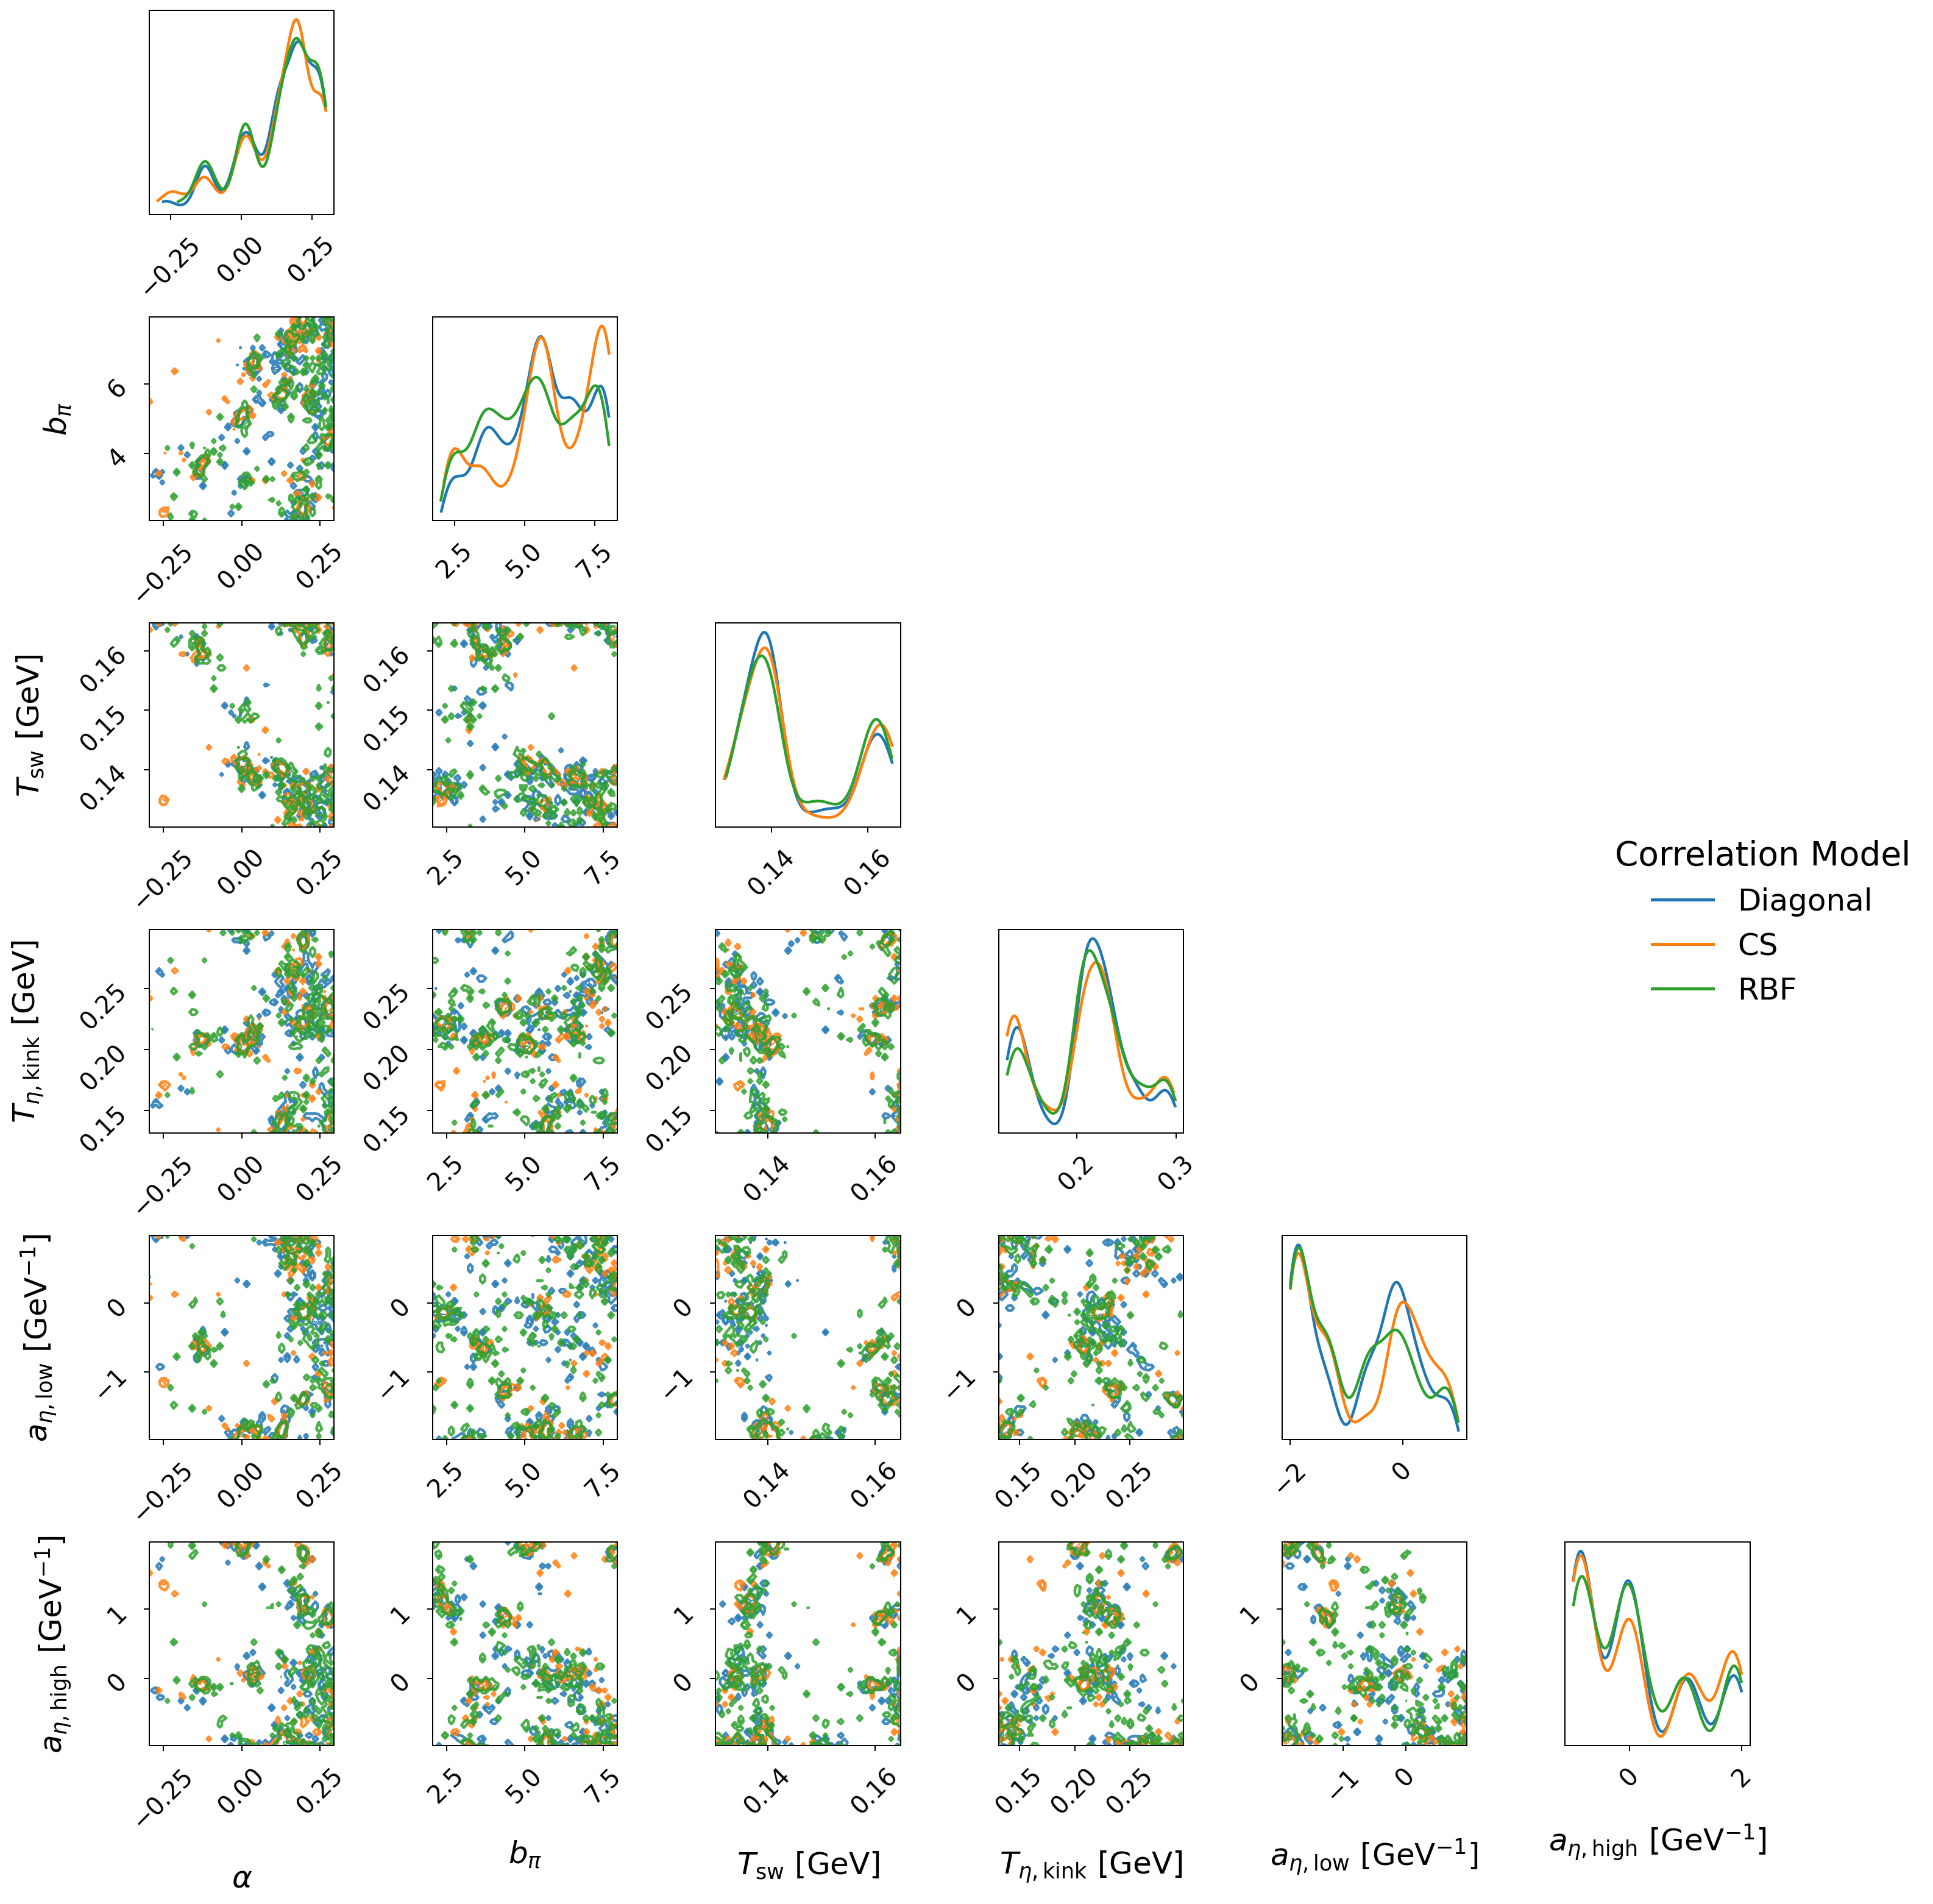
\includegraphics[width=0.48\textwidth]{img/corner_all_models_2-menos.png}

\vspace{0.15cm}

\tiny
Posterior distributions obtained using the Diagonal, Compound Symmetry (CS), and RBF experimental covariance models.
\end{frame}

%--------------------------------------------------------

\begin{frame}
\frametitle{Preliminary Results}

\centering
\scriptsize
ALICE Pb--Pb $\sqrt{s_{NN}}=2.76$ TeV, universal spectra calibration

HEPData: \texttt{ins1222333}

\vspace{0.2cm}

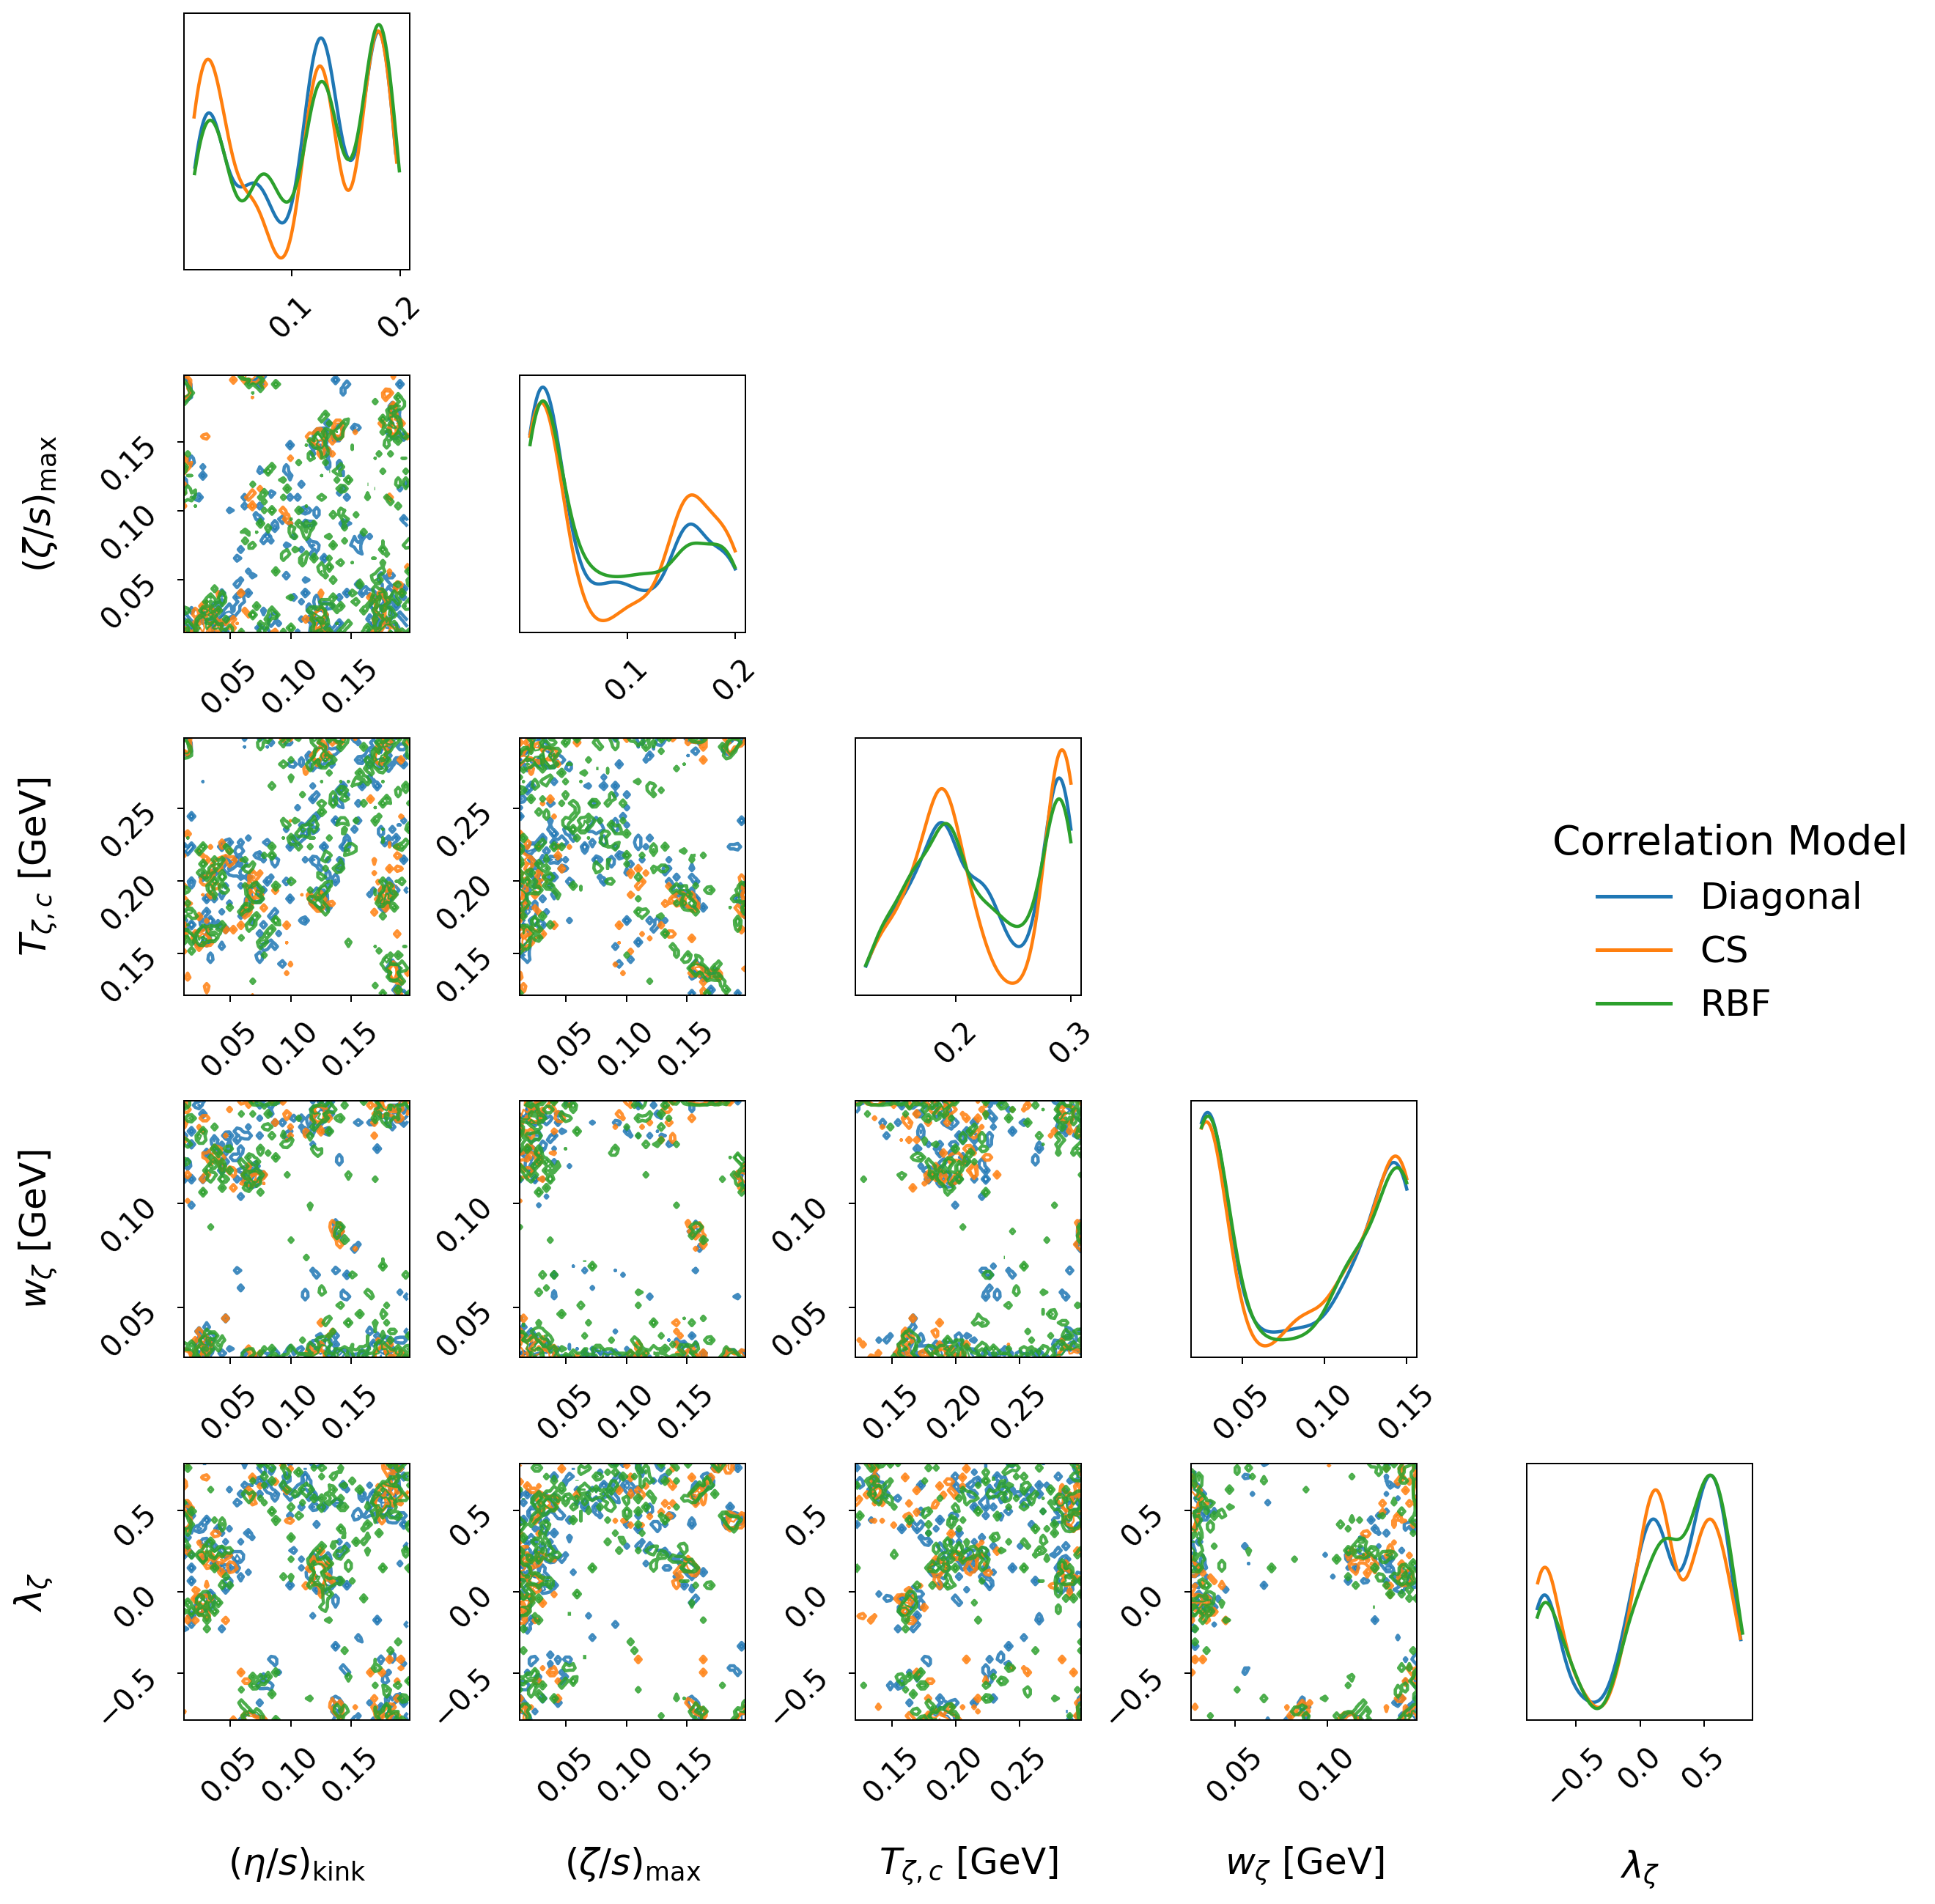
\includegraphics[height=0.74\textheight,keepaspectratio]{img/corner_all_models_3-menos.png}

\vspace{0.15cm}

\tiny
Posterior distributions obtained using the Diagonal, Compound Symmetry (CS), and RBF experimental covariance models.
\end{frame}
%--------------------------------------------------------

\begin{frame}
\frametitle{Preliminary Results}

\begin{columns}[T]

%====================================================
% COLUMN 1
%====================================================

\column{0.42\textwidth}

\centering

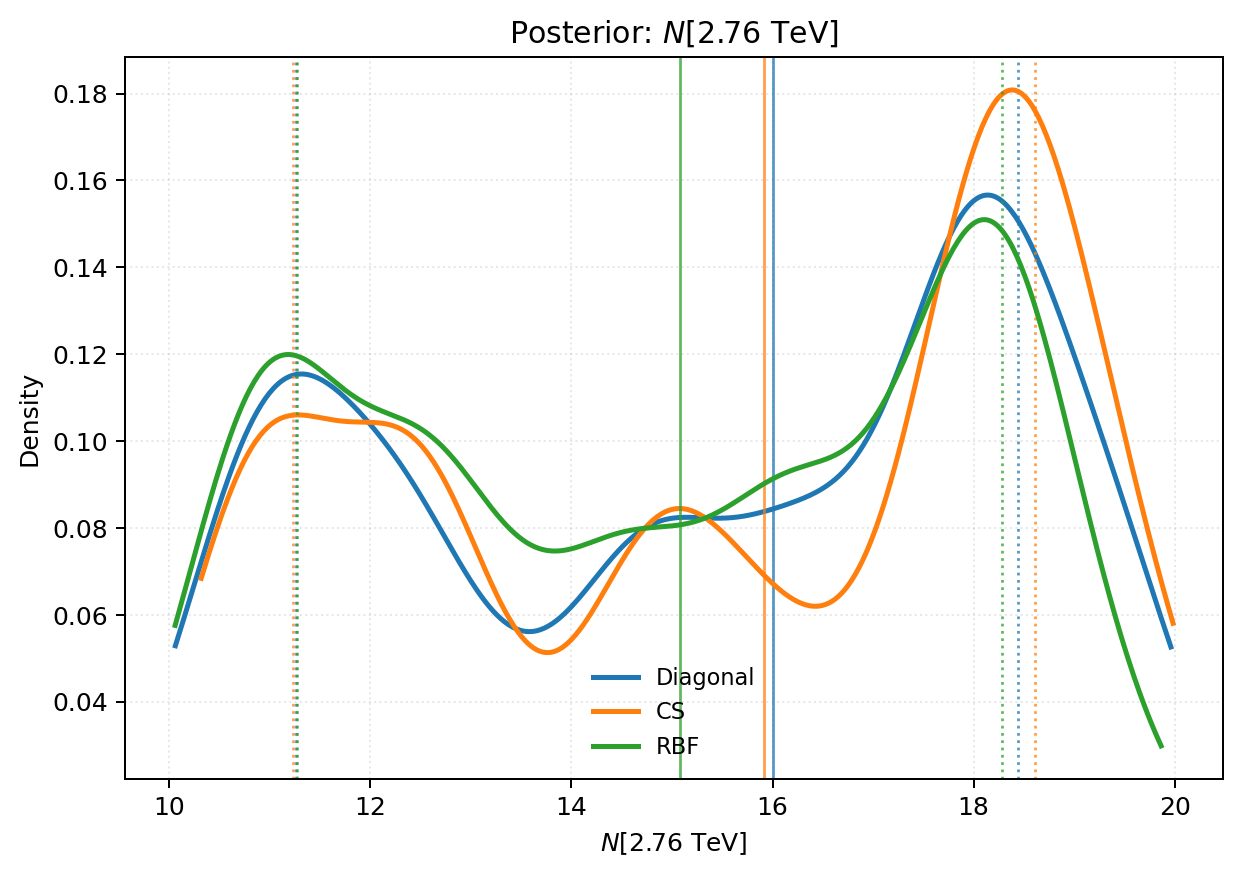
\includegraphics[width=\linewidth]{img/posterior_parameter_01.png}

\vspace{0.18cm}

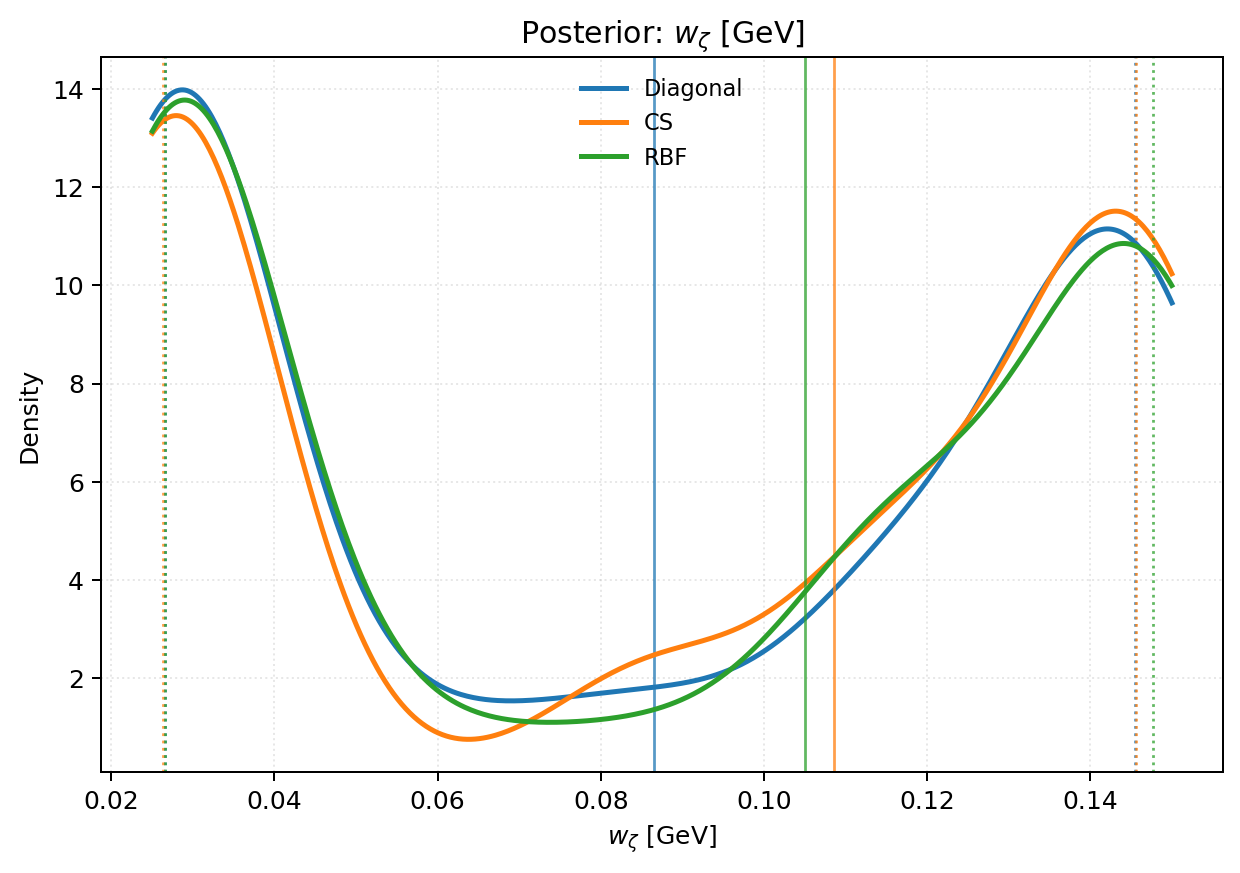
\includegraphics[width=\linewidth]{img/posterior_parameter_14.png}

%====================================================
% COLUMN 2
%====================================================

\column{0.38\textwidth}

\centering

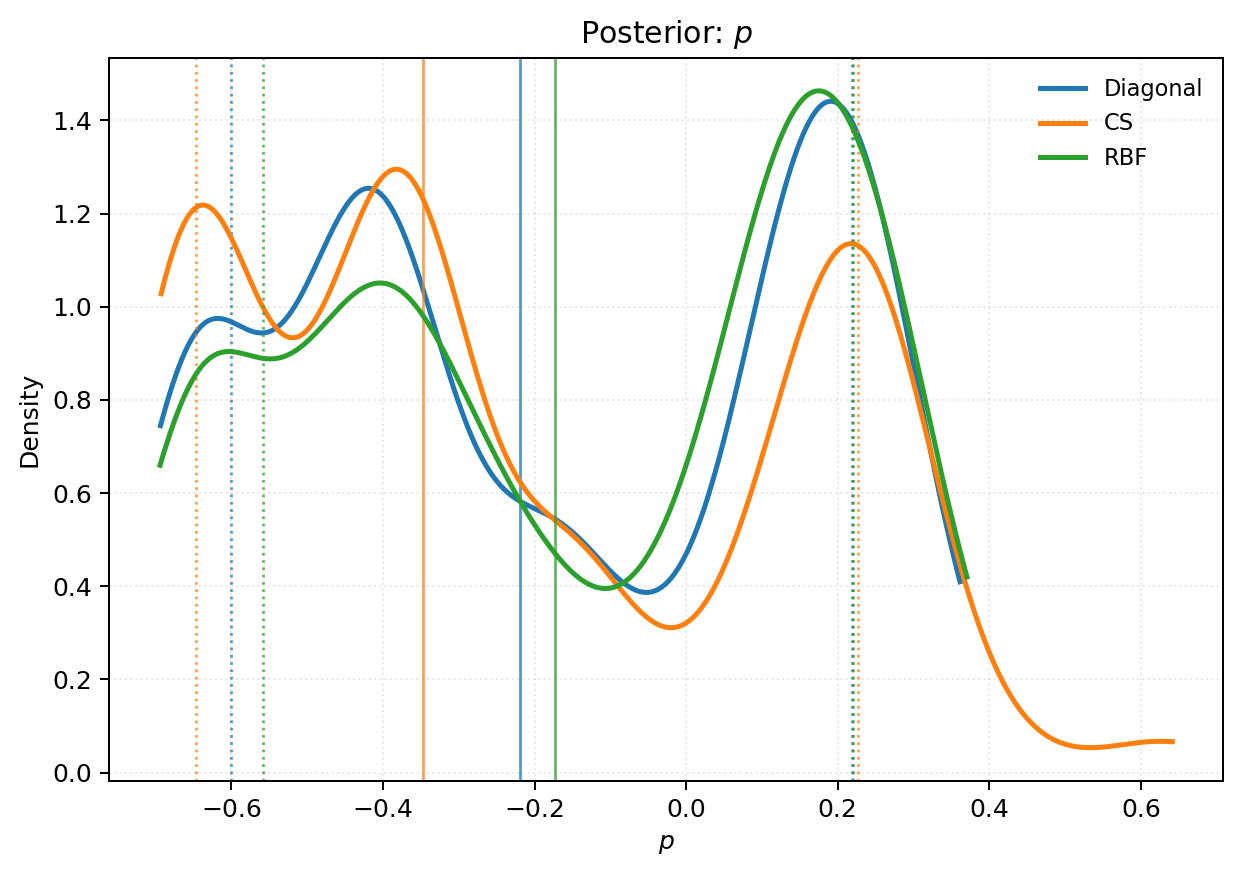
\includegraphics[width=\linewidth]{img/posterior_parameter_02.png}

\vspace{0.72cm}

\scriptsize
\renewcommand{\arraystretch}{1.18}

\begin{tabular}{lr}
\hline
\multicolumn{2}{c}{\textbf{Largest posterior shifts}}\\
\hline
\textbf{Parameter} & \textbf{Max shift}\\
\hline
$p$ & $0.515\sigma$\\
$w_{\zeta}$ & $0.418\sigma$\\
$N$ & $0.307\sigma$\\
\hline
\end{tabular}

\vspace{0.25cm}

\tiny
Largest normalized median shifts among the 17 inferred parameters.

%====================================================
% COLUMN 3
%====================================================

\column{0.20\textwidth}

\centering

% \large
% \textbf{Global comparison }

\vspace{0.68cm}

{\fontsize{11}{12}\selectfont\bfseries
14/17
}

\vspace{0.08cm}

\tiny
parameters with\\
$\Delta<0.3\sigma$

\vspace{0.38cm}

{\fontsize{11}{12}\selectfont\bfseries
3/17
}

\vspace{0.08cm}

\tiny
parameters with\\
$\Delta>0.3\sigma$

\vfill
\vspace{0.24cm}

\tiny
Changing the experimental covariance structure (Diagonal → CS → RBF) produces no statistically significant change in the inferred posterior for the Universal Scaled Spectra calibration, with posterior shifts remaining below $0.6\sigma$ across all inferred parameters.
\end{columns}

\vspace{0.12cm}

\centering
\tiny
Posterior comparison for ALICE Pb--Pb $\sqrt{s_{NN}}=2.76$ TeV, universal spectra calibration.
\end{frame}
%--------------------------------------------------------
\section{Next Steps}

\begin{frame}
\frametitle{Next Steps}

\begin{columns}[c]

\column{0.22\textwidth}

\centering

\includegraphics[width=0.70\linewidth]{img/jetscape_logo.png}

\vspace{0.15cm}

\scriptsize
The JETSCAPE\\
Collaboration

\column{0.78\textwidth}

\small

\textbf{Planned extensions of this work}

\vspace{0.2cm}

\begin{itemize}
    
    \item Au--Au collisions at $\sqrt{s_{NN}}=200$ GeV
    \item Multi-experiment calibration (STAR, PHENIX, PHOBOS and BRAHMS)
    \item Reproduce the JETSCAPE Bayesian analysis (Mankolli \textit{et al.}, 2026) evaluating the impact of correlated experimental uncertainties arXiv:2601.17234 
\end{itemize}

\vspace{0.3cm}

\textbf{Target reference}

\smallskip

% \texttt{[nucl-ex]}

\end{columns}

\vfill

\centering
\scriptsize

\end{frame}
%----------------------------------------------------------------------------------------
% AGRADECIMENTOS
%----------------------------------------------------------------------------------------

\begin{frame}[plain]

\begin{center}

\vspace{1.5cm}

{\Huge
\textcolor{titleRed}{
\textbf{Thank you!}
}
}

\vspace{0.7cm}

\vfill

\begin{figure}
\centering

\includegraphics[height=1cm]{logo_ifusp.png}
\hspace{0.5cm}

\includegraphics[height=1.2cm]{logo_ifna.png}
\hspace{0.5cm}

\includegraphics[height=1.1cm]{logo_cbpf.jpg}
\hspace{0.5cm}
\raisebox{1mm}{
\includegraphics[height=0.9cm]{logo_cnpq.jpg}}

\end{figure}

\vspace{0.2cm}

{\small
CNPq -- Project No. 132734/2025-7
}

\end{center}

\end{frame}

%----------------------------------------------------------------------------------------

% REFERÊNCIAS

%----------------------------------------------------------------------------------------

% \begin{frame}[allowframebreaks]


% \frametitle{References}

% \printbibliography

% \end{frame}
%----------------------------------------------------------------------------------------
% FIM
%----------------------------------------------------------------------------------------
\end{document}